%\documentclass[11pt,a4paper,twoside]{tesis}
% SI NO PENSAS IMPRIMIRLO EN FORMATO LIBRO PODES USAR
\documentclass[11pt,a4paper]{tesis}

\usepackage{graphicx}
\usepackage[utf8]{inputenc}
\usepackage[spanish]{babel}
\usepackage[left=3cm,right=3cm,bottom=3.5cm,top=3.5cm]{geometry}

\usepackage{color}
\usepackage{solucion}
\usepackage{multicol}
\usepackage{algorithm}
\usepackage{algorithmic}
\usepackage{xcolor}
\usepackage{colortbl}
\usepackage{lscape}
\usepackage{longtable}
\usepackage{amsmath}
\usepackage{amssymb}
\renewcommand{\algorithmicrequire}{\textbf{Input:}}
\renewcommand{\algorithmicensure}{\textbf{Output:}}
\begin{document}

%%%% CARATULA
% Comentar y descomentar según corresponda
\def\titulo{Licenciado }
\def\autor{Amit Stein, Juan Andrés Knebel}
\def\tituloTesis{Composite Retrival: \mbox{Algo}}
\def\runtitulo{Composite Retrival en español}
\def\runtitle{Composite Retrival en ingles}
\def\director{Obi-Wan Kenobi}
\def\codirector{Master Yoda}
\def\lugar{Buenos Aires, 2014}
%\newcommand{\HRule}{\rule{\linewidth}{0.2mm}}
%
\thispagestyle{empty}

\begin{center}\leavevmode

\vspace{-2cm}

\begin{tabular}{l}

\includegraphics[width=2.6cm]{logofcen.pdf}
\end{tabular}


{\large \sc Universidad de Buenos Aires

Facultad de Ciencias Exactas y Naturales

Departamento de Computaci\'on}

\vspace{6.0cm}

%\vspace{3.0cm}
%{
%\Large \color{red}
%\begin{tabular}{|p{2cm}cp{2cm}|}
%\hline
%& Pre-Final Version: \today &\\
%\hline
%\end{tabular}
%}
%\vspace{2.5cm}

{\huge\bf \tituloTesis}

\vspace{2cm}

{\large Tesis presentada para optar al t\'{\i}tulo de\\
\titulo en Ciencias de la Computaci\'on}

\vspace{2cm}

{\Large \autor}

\end{center}

\vfill

{\large

{Director: \director}

\vspace{.2cm}

{Codirector: \codirector}

{Codirector: \codirectordos}

\vspace{.2cm}

\lugar
}

\newpage\thispagestyle{empty}


%%%% ABSTRACTS, AGRADECIMIENTOS Y DEDICATORIA
\frontmatter
\pagestyle{empty}
%%\begin{center}
%\large \bf \runtitulo
%\end{center}
%\vspace{1cm}
\chapter*{\runtitulo}

\noindent Las búsquedas tradicionales nos ofrecen una solución que solo tiene en cuenta un atributo de los elementos y no la relación que éstos tienen con el resto del universo. Las mismas nos ofrecen un lista ordenada de resultados que cumplen con el criterio elegido en mayor o menos medida, ocasionando que muchas veces se necesite reformular la consulta original para así lograr la solución que el usuario quiere encontrar.\\
Los algoritmos de agrupación clásicos o clustering generan conjuntos de soluciones, que al igual que las búsquedas tradicionales, los elementos dentro de cada conjunto o cluster cumplen con el criterio elegido y además entre sí comparten alguna propiedad (generalmente una similitud o distancia), pero no se analiza ningún tipo de Complementaridad entre los elementos. La relación entre los cluster no es analizada ocacionando que entre ellos sean muy similares o diferentes dependiendo del universo en el cuál se encuentre trabajando.\\
Es por eso que surge \textbf{Composite Retrieval}, su objetivo es agrupar elementos en cluster bajo un mismo atributo, al mismo tiempo que éstos son complementarios entre sí por algún atributo definido previamente. A diferencia de las anteriores técnicas se permite elegir el grado de interdepencia entre los conjuntos generados permitiendo, según el caso, que los conjuntos que componen la solución sean más o menos parecidos facilitando al usuario la elección de un grupo de elementos que satisfagan su consulta original.

\bigskip

\noindent\textbf{Palabras claves:} Composite Retrieval, Similitud, Complementaridad, Búsqueda Tabú, Generación de Bundles, Agrupamiento.

%\cleardoublepage
%%\begin{center}
%\large \bf \runtitulo
%\end{center}
%\vspace{1cm}
\chapter*{\runtitulo}

\noindent Las búsquedas tradicionales ofrecen soluciones que solo tienen en cuenta un solo atributo de los elementos y no la relación que estos tienen con el resto del universo. Las mismas suelen ofrecer una lista ordenada de resultados relacionadas con
el criterio utilizado. Ocasionando, muchas veces, re formular la consulta original para así lograr una solución adecuada al criterio de búsqueda elegido previamente.\\
Los algoritmos de agrupación clásicos o clustering generan conjuntos de soluciones, al igual que las búsquedas tradicionales, en los cuales los elementos dentro de cada conjunto (o cluster) tiene una relación directa con la búsqueda original y además se encuentran relacionados de alguna manera (generalmente una similitud o distancia). Aún así, éstas soluciones no tienen en cuenta ningún atributo que represente la complementaridad que existe entre los elementos, ocasionando que la solución encontrada contenga conjuntos de objetos muy similares sin diversidad. La relación entre los cluster no es sujeto de ningún análisis en estos algoritmos. En orden de lograr una solución con mayor diversidad (evitar cluster similares) y que cumpla las expectativas del usuario, debería existir un análisis entre los clusters.\\
Como respuesta a éste último comportamiento surge Composite Retrieval of Diverse and Complementary Bundles \cite{compositeRetrival}, su objetivo es agrupar elementos en bundles en los cuales los elementos dentro de ellos se encuentran relacionados internamente bajo algún criterio de similitud y a la vez sean complementarios de forma tal que satisfaga las expectativas del usuario y no tenga la necesidad de realizar una nueva intervención logrando así una mejor experiencia de búsqueda.\\
En este trabajo se tomaron las ideas ya desarrolladas previamente en \cite{compositeRetrival}, se propuso un nuevo algoritmo, nuevas mejoras y enfoques en orden de mejorar los resultados que se obtuvieron originalmente y los tiempos de ejecución para instancias más grandes. Las nuevas aplicaciones se aplicaron a la resolución de búsquedas sobre una base de datos de artículos científicos pertenecientes a la Ingeniería de Software \cite{dataDrive} y sobre una instancia conformada por atracciones turísticas de Europa.

\bigskip

\noindent\textbf{Palabras claves:} Composite Retrieval, Similitud, Complementaridad, Búsqueda Tabú, Generación de paquetes, Agrupamiento.

%\cleardoublepage
%\chapter*{Agradecimientos}

\noindent A Laura que estuvo a mi lado
\noindent A mis padres, a Abigail y René y a Edith que me acompañaron y ayudaron durante toda la carrera y A Mila y Florián que lo hicieron este último tramo. 
\noindent a todos los profesores y ayudantes del DC y en especial a Paula, Isabel y Estebán por todo lo enseñado.
\noindent A Dario, Julio y Sebastián con los que además de compañeros nos hicimos buenos amigos.
\noindent A Anita que me acompañó y me apoyó en todos estos últimos años de mi vida y que hace que cada día sea más lindo que otro.
\noindent A todo mi familia por todo lo que me dieron sin pedir nada: Hugo, Graciela, Nicolas, Luciana, Marco, Blas, Julia, Carlita.
\noindent A mis amigos de siempre de Bahía Blanca por bancarme en todas.
\noindent A Ezequiel Cura que aunque solo cursamos una sola vez y no veamos poco, es un gran amigo.
\noindent A mis compañeros de trabajo de Technisys que se aguantaron tantas charlas de este trabajo. % OPCIONAL: comentar si no se quiere

%\cleardoublepage
%\hfill \textit{A Nestor y Chavez que nos cuidan y guian desde arriba}  % OPCIONAL: comentar si no se quiere

\cleardoublepage
\tableofcontents

\mainmatter
\pagestyle{headings}

%%%% ACA VA EL CONTENIDO DE LA TESIS

\chapter{Introducción}
\section{Estado Actual de las Búsquedas}
{\begin{small}%
\begin{flushright}%
\it An algorithm must be seen to be believed.\\Donald Knuth.
\end{flushright}%
\end{small}%
\vspace{.5cm}}
Las búsquedas son acciones que se llevan a cabo con el fin de hallar elementos. Para lograr el objetivo el usuario debe ingresar frases o términos relacionados a fin de encontrar los resultados deseados. A lo largo del desarrollo de Internet las búsquedas fueron adquiriendo cada vez más importancia por la enorme cantidad de información que cada día se almacena en los distintos servidores a lo largo del planeta.\\
En un principio los algoritmos utilizados eran más simples o se basaban únicamente en buscar coincidencias exactas de las frases ingresadas en los elementos a buscar. Con el paso del tiempo las estrategias fueron evolucionando y adaptándose, con el objetivo de devolverle al usuario resultados más completos y que a la vez sean relevantes.\\
La \textbf{Recuperación de la Información} (IR por Information Retrieval en inglés), es la actividad de obtener información relevante de una inmensa colección de datos y con criterios de lo más variados, desde el resultado de la final del mundial de fútbol, los libros de un autor y hasta el mail de la confirmación de una compra.\\
Los motores de búsquedas de la web como Google, Yahoo y otros, son los clásicos ejemplos de una aplicación de IR. El proceso de búsqueda comienza cuando el usuario ingresa una consulta de la que el buscador devuelve una colección de elementos que coinciden con el criterio de búsqueda. En general lo que ocurre es que son varios los elementos del universo que concuerdan pero con grados de relevancia diferentes (ranking de resultados) que se utiliza para ordenar la colección de elementos devueltos. Para obtener el ranking de resultados los sistemas de IR trabajan con una representación lógica de los elementos que incluye los metadatos necesarios para operar sobre ellos. La desventaja de los ranking de resultados es que únicamente se compara la consulta de la búsqueda con los metadatos de los elementos, dejando de lado el análisis de los elementos entre sí y conviritiendo, en ocasiones, al proceso en una acción tediosa y repetitiva ya que el usuario deberá cambiar la consulta original y explorar la colección de elementos hasta lograr encontrar el o los elementos deseado.\\
En el  artículo \textbf{Composite Retrieval of Diverse and Complementary Bundles}\cite{compositeRetrival} se propone presentar una lista de grupos de elementos, en lugar de entregar una lista vertical de los mismos. Cada grupo deberá estar relacionado internamente bajo el criterio de similitud elegido y la lista ordenada de forma lógica con la finalidad de que uno o más conjuntos satisfagan las expectativas del usuario sin necesidad de una nueva intervención para refinar su búsqueda para lograr una mejor experiencia de búsqueda.\\
La finalidad de este trabajo es devolver los resultados de las búsquedas como plantea el artículo \textbf{Composite Retrieval of Diverse and Complementary Bundles} para ello se analizaron e implementaron los algoritmos de agrupamiento (o clustering) que realizan la tarea de agrupar en conjuntos disjuntos a elementos que pertenecen a una misma clase. Las dos técnicas más usadas son agrupamiento jerárquico y no jerárquico. La primera a su vez se puede dividir en dos tipos, aglomerativos donde todos los elementos comienzan como un cluster para luego mezclarse entre ellos y divisivos en el cual se comienza con un único grupo y se comienza a dividir. Para las decisiones de unir o dividir se usan medidas de similitud o disimilitud de los elementos del conjunto. Para la segunda técnica de clusterización se definen previamente cuales serán los grupos finales y se van asignado los demás elementos al grupo que correspondan. Además de las técnicas de clusterización, se desarrollaron heurísticas para buscar una solución mejor.\\
\section{Motivación}
Planear un viaje típicamente requiere realizar múltiples búsquedas en distintos motores para recabar la información de los diferentes destinos que se quiere visitar, las distancias geográficas, los precios de las atracción o leer opiniones acerca de los destinos seleccionados, entre otros.\\
En una búsqueda típica los resultados obtenidos son una larga lista ordenada por la relevancia del criterio de la consulta. Este tipo de soluciones no otorgan respuestas que relacionen el criterio buscado con los demás elementos de la lista resultante.\\
Otro ejemplo es el caso en el que un cliente de una tienda online de venta de discos que le gusta escuchar música de diferentes países, cuenta con un presupuesto limitado y no está interesado en un ningún género musical específico, pero si quiere comprar un conjunto de discos que pertenezcan al mismo género musical. El cliente al comenzar su búsqueda obtendría una lista parecida a la siguiente:
\begin{itemize}
  \item Physical Graffiti - Led Zeppelin
  \item Led Zeppelin - Led Zeppelin
  \item It's Hard - The Who
  \item Perfect Strangers - Deep Purple
  \item El Cielo Puede Esperar - Attaque 77
  \item Wheels of Fire - Cream
  \item Confesiones de Invierno - Sui Generis
  \item The White Album - The Beatles
  \item Innuendo - Queen
  \item Sticky Fingers - The Rolling Stones
  \item Kamikaze - Luis Alberto Spinetta
\end{itemize}

De la lista obtenida el usuario deberá seleccionar aquellos discos que sean de su interes con el posible error de elegir más de un disco del mismo origen. Segundo, deberá ir agregando y eliminando de su lista manualmente en el caso que la elección de un disco superase el presupuesto que él posee. Tercero, no necesariamente elegirá el mejor subconjunto de discos que maximice su presupuesto y a su vez el origen de los discos sean distintos.\\
Para este tipo de búsquedas la solución que se propone está pensada para aquellas consultas que requieren obtener un conjunto de elementos que se relacionan como respuesta. Se podría realizar una clusterización de los resultados pero, en las técnicas tradicionales la agrupación se hace por la similitud entre ítems. En el ejemplo de los discos con una clusterización tradicional, donde la similitud sea el género musical, seguramente se generen tantos cluster como géneros de discos existan y en cada cluster se encontrarán todos los discos de ese género. Una vez obtenido el resultado se deberá explorar todos los clusters para elegir los discos.\\
En cambio si se aplicase las técnicas mencionadas en \textit{``Composite Retrieval of Diverse and Complementary Bundles''} las soluciones obtenidas se ajustarían al presupuesto y cada uno de los ítems dentro del bundle (es el nombre que se le da al agrupamiento de ítems) sean complementarios entre sí, de modo tal, que el usuario pordrá optar por cualquier bundle de la solución y estar seguro que su elección cumple con su objetivo inicial, que pertenece a un mismo género musical y exista variedad en la elección.\\
Si en el ejemplo de la tienda de discos se establece la complementariedad del atributo que refleja el origen de la banda y se establece un presupuesto máximo a cada bundle, una solución posible sería:
\begin{itemize}
  \item Bundle 1:
  \begin{itemize}
    \item Physical Graffiti - Led Zeppelin (Inglaterra)
    \item After chabón - Sumo (Argentina)
    \item Back in Black - AC/DC (Estados Unidos)
  \end{itemize}
  \item Bundle 2:
  \begin{itemize}
    \item Natty Dread - Bob Marley (Jamaica)
    \item El ritual de la Banana - Los Pericos (Argentina)
    \item Labour of Love - UB40 (Inglaterra)
  \end{itemize}
	  \item Bundle 3:
  \begin{itemize}
    \item Ramones - Ramones (Estados Unidos)
    \item El Cielo Puede Esperar - Attaque 77 (Argentina)
    \item Sandinista! - The Clash (Inglaterra)
  \end{itemize}
\end{itemize}
Lo que se quiere lograr en los ejemplos descriptos y en cualquier otro problema similar de búsquedas es otorgarle al usuario un conjunto de bundles que cumplan siempre con las siguientes propiedades: 
\begin{itemize}
  \item \textbf{Cubrimiento}: Maximizar la cantidad de elementos en el bundle.
  \item \textbf{Compatibilidad}: Los elementos del bundle deben ser similares.
  \item \textbf{Validez}: El costo total de los elementos del bundle no debe superar el presupuesto.
  \item \textbf{Diversificada}: Los bundles entre si deben ser diversos.
\end{itemize}

\chapter{Búsquedas}
La instancia seleccionada para realizar las pruebas de lo propuesto en este trabajo es sobre la base de datos de los artículos de \textit{\textquotedblleft A Data-Driven Journey through Software Engineering Research\textquotedblright}\cite{dataDrive}. La decisión de utilizar esta base de datos es por la completitud de la información y que la cantidad de elementos que contiene requiere de algoritmos eficientes. La base de datos contiene cerca de $7800$ artículos, de los que se tiene los autores que participaron en ellos, en la conferencia que fueron presentados y lo más importante es que se cuenta con una clasificación ya realizada de los tópicos a los que hacen referencia cada uno de ellos. Ésta última característica es llamada \texttt{topicProfile} y esta expresada en porcentajes para cada uno de tópicos que son tratados. De los $9800$ autores se tiene la información de que a universidad pertenecen y además de cada una de las universidades se sabe a que región pertenece cada una.\\

El \texttt{topicProfile} es muy importante porque permitirá definir la similitud no sólo entre los artículos, sino que también entre los autores y las universidades de la base da datos de una manera prácticamente directa.\\

Para las pruebas, los criterios de las búsquedas que se realizaron sobre la base de datos se concibieron a partir de lo que se consideró que tiene un interés general. Por ejemplo, quiénes son los autores que escribieron artículos similares de distintas universidades o las universidades de diferentes regiones donde se escribieron artículo de los mismos tópicos.\\
Por lo establecido en \cite{compositeRetrival} para las búsquedas se deben realizar las siguientes definiciones:
\begin{itemize}
  \item \textbf{Similitud}: Función que dado dos ítems devuelve la similitud entre estos.
  \item \textbf{Costo}: Función que dado un ítem devuelve el costo del mismo.
  \item \textbf{Presupuesto}: El presupuesto que se tiene, el cual no podrá ser excedido por ningún bundle.
  \item \textbf{Complmentariedad}: Propiedad del ítem que es único en cada bundle.
\end{itemize}
Para todas las búsquedas, sin importar el ítem que sea (artículo, autores o universidades),  se definió que el costo de cada ítem sea de una unidad y que el presupuesto para cada búsqueda es de cinco unidades. Por lo que en todos los resultados se obtienen bundles que contienen como máximo cinco ítems; además se deicidió que sean diez los bundles devueltos en cada búsqueda. El motivo es para que sea fácil para un humano valorizar el resultado propuesto. Entonces de aquí en adelante para cada criterio de búsqueda se deben definir únicamente la función de similitud y la propiedad de complementariedad.\\
Como se mencionó anteriormente, en la base de datos cada artículo cuenta con su \texttt{Topic Profile}. El \texttt{Topic Profile} define el perfil de cada artículo asignándole un porcentaje a cada tópico que se hace referencia. En el caso del artículo \texttt{A Cognitive-Based Mechanism for Constructing Software Inspection Teams} el \texttt{Topic Profile} se compone por los tópicos  REQUIREMENTS, RELIABILITY, TESTING y SOFTWARE QUALITY el porcentaje de cada uno de estos es 71.43 \%, 17.86 \%, 7.14 \% y 3.57 \% respectivamente. \\
De los autores no se cuenta con una información directa que defina el perfil. Por lo tanto el perfil de los autores se genera a partir de los artículos que escribieron. Para definir el perfil de las universidades se aplicó el perfil de los autores definidos anteriormente. Más adelante se verá como se utilizan los perfiles para definir la función de similitud entre los ítems. A continuación se detallan las consultas realizadas en este trabajo.\\
Se utilizaron los siguientes criterios a las consultas que se hicieron en la base de datos, en los cuales la función costo para todos los elementos se defino con la constante 1 y el presupuesto de 5. Se decidió así porque no tiene sentido asociarle un costo a los artículos, autores, universidades y solo nos interesa que el bundle tengo como máximo un número fijo de elementos. Entonces de aquí en adelante para cada criterio solo resta definir la función de similitud y la propiedad de complementariedad.

\section{Artículos de diferentes conferencias}\label{bus:papSimDisLug}
Generar una solución, en el que cada bundle contenga artículos similares que se hayan presentado en distintas conferencias.\\
\begin{itemize}
  \item \textbf{Similitud}: Función que compara el perfil de cada artículo.
  \item \textbf{Complementariedad}: Lugar dónde fue presentado.
\end{itemize}

\section{Autores de distintas universidades}
Solución de bundles en el que cada uno contiene autores similares de distinta universidad de afiliación.\\
\begin{itemize}
  \item \textbf{Similitud}: Función que compara el perfil de los autores.
  \item \textbf{Complementariedad}: Universidad de pertenencia del autor.
\end{itemize}

\section{Instituciones de diferentes regiones}
En este caso, la búsqueda es para instituciones de diferentes regiones. 
\begin{itemize}
  \item \textbf{Similitud}: Función que compara el perfil de las instituciones.
  \item \textbf{Complementariedad}: Región de la institución.
\end{itemize}

Como se menciona antes, la base de datos cuenta con un \texttt{Topic Profile} de cada artículo que es un porcentaje del tema al que hace referencia. Esto se puede transformar a un vector de $n$ dimensiones en dónde cada posición representa un tópico diferente, entonces para cada artículo se obtiene un vector de la misma dimensión. Ésto es clave para la generación de la similitud entre los artículos.\\
Para los autores no se cuenta con información más allá de los artículos que escribieron, pero sólo con eso alcanza para poder generar un perfil de autores, por lo tanto para cada autor se hace la suma vectorial de cada uno de los \texttt{Topic Profile} de los artículos en los cuales participó y con eso obtenemos el \texttt{Topic Profile de Autores}.Para obtener el perfil de las universidades se aplicó el mismo criterio que para los autores, de hacer la suma vectorial de cada uno de los \texttt{Topic Profile de Autores} pertenecientes a la misma universidad y así generar el \texttt{Topic Profile de Universidades}. En ambos casos se aplica la normalización sobre los vectores resultantes.

Ejemplo de los perfiles de los elementos:

\begin{description}
 \item[Artículo - Topic Profile - Autores]
 \item Artículo 1 - $[$0.20, 0.40, 0.40, 0.00$]$ - Autor 1, Autor 2, Autor 3
 \item Artículo 2 - $[$0.30, 0.70, 0.00, 0.00$]$ - Autor 2, Autor 3
 \item Artículo 3 - $[$0.00, 0.10, 0.00, 0.90$]$ - Autor 2
 \item Artículo 4 - $[$0.00, 0.00, 1.00, 0.00$]$ - Autor 1, Autor 3
\end{description}

\begin{description}
 \item[Autor - Topic Profile - Universidad]
 \item Autor 1 - $[$0.14, 0.27, 0.95, 0.00$]$ - Universidad 1
 \item Autor 2 - $[$0.30, 0.74, 0.25, 0.55$]$ - Universidad 2
 \item Autor 3 - $[$0.27, 0.60, 0.76, 0.0$]$ - Universidad 2
\end{description}

\begin{description}
 \item[Universidad - Topic Profile]
 \item Universidad 1 - $[$0.14, 0.27, 0.95, 0.00$]$
 \item Universidad 2 - $[$0.31, 0.72, 0.54, 0.30$]$
\end{description}

\section{Función de similitud}
La similitud se emplea para comparar dos objetos y determinar qué tan parecido son entre si. En este trabajo para determinar la similitud entre los objetos es por la medida conocida como \textbf{similitud coseno}. Esta es una medida de similitud entre dos vectores en un espacio vectorial provisto de un producto escalar que mide el coseno del ángulo comprendido entre ellos. El coseno para el ángulo cero es 1, es menor a 1 para cualquier otro ángulo y es 0 cuando los vectores son ortogonales. De esta forma lo que define la similitud de los vectores es la orientación y no así la magnitud.\\
Entonces se define la función de similitud $S(V_i, V_j)$ para los vectores $V_i$ y $V_j$ a partir del producto escalar\\

\begin{equation} \label{eq:angulovectorial}
\cos(\theta) =  \dfrac{\overrightarrow{U} . \overrightarrow{V}}{\overrightarrow{\lVert V\lVert}.\overrightarrow{\lVert U\lVert}}
\end{equation}

Para esta instancia los objetos (ahora artículos, autores o universidades) son representados por vectores, donde cada dimensión corresponde a un tópico y el valor se corresponde con el valor del tópico del objeto según la base de datos \cite{dataDrive}. Por lo tanto el objeto $a$ se representa con el vector $V_a = [v_1,v_2,...,v_n]$, donde $N$ es la cantidad de tópicos y cumple con las siguientes propiedades:
\begin{enumerate}
 \item $v_i \geq 0$
 \item $\sum{v_i} = 1$
\end{enumerate}

Como los componentes de todos los vectores son mayor o igual a cero se obtiene que $0\leq\cos(\theta)\leq1$, que implica que $S(V_i, V_j) \in \left[0, 1\right]$.\\

\begin{figure}[H]
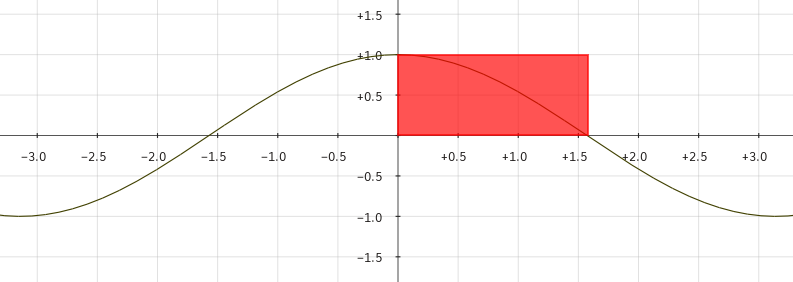
\includegraphics[width=0.8\textwidth]{img/coseno.png}
\caption{Comportamiento de la función $\cos$. En rojo la región que pertenece a la función de similitud}
\label{bus:img-coseno}
\end{figure}

Dos vectores proporcionales tiene la misma dirección y el ángulo entre ellos es cero, entonces la función de similitud es 1. Lo que significa que esta medida de similitud no considera el peso de cada tópico, por lo tanto no diferencia entre un artículo profesional y un artículo de un diario que cubre el mismo tópico. Esta debilidad de la medida basada en el ángulo no interfiere en este trabajo por la segunda propiedad de los vectores del problema, porque para que dos vectores sean proporcionalmente iguales tienen que ser idénticos y en tal caso es correcto que la similitud entre ellos sea 1. 
\chapter{Desarrollo}
\section{Modelo}
Dado el conjunto de items I y la función de similitud \textbf{S}: IxI$\rightarrow$R[0;1]. El problema lo podemos representar como un grafo 
con peso en las aristas, en el cuál los vertices son los items y el peso de las aristas es la similitud entres estos.
\section{Problema}
El problema de obtener el conjunto de bundles que máximiza la función objetivo se puede considerar como un problema
de clusterización en el cual la calidad de los cluster esta dado por la cohesión de los items que lo componen y la
separación entre cluster con menos similitud.
Las diferencias con los problemas tipicos de clusterización son:
\begin{enumerate}
 \item La cantidad de items en un bundle esta limitada por el presupuesto.
 \item En el bundle no puede existir más de un item con el mismo atributo de complementaridad.
\end{enumerate}
\section{Función de similitud}
La similitud \textbf{S} del conjunto de los items I, \textbf{S}: IxI$\rightarrow$R[0;1], entre los papers esta dado por la comparación del perfil de cada uno. El perfil del paper se obtiene del topic profile, para hacer la comparación se represento el topic profile cómo un vector de $N$ dimensiones, donde $N$ es la cantidad de tópicos, normalizados ya que cada compenente representa un porcentaje del tema al que pertenece.\\
Dados estos vectores calcular la similitud entre los papers es la distancia angular entre ellos. Los vectores que formen un ángulo cercano a $0$\textdegree representan una similitud alta entre los perfiles, mientras que un ángulo cercano a $90$\textdegree dos perfiles ortogonales o diferentes.\\
\subsection{Cálculo de ángulos}
Lo siguiente demostración es en $\Re^{2}$ por ser visualmente más fácil de exponer, es fácilemente extensible a $\Re^{n}$.\\
La función del ángulo entre los vectores $V, U$ es:\\
$$\cos(\hat{\theta}) = \dfrac{\overrightarrow{V}.\overrightarrow{U}}{\overrightarrow{\lVert V\lVert}.\overrightarrow{\lVert U\lVert}}$$

En este gráfico se visualiza el comportamiento de la función $\cos$\\
\begin{figure}[H]
\centering
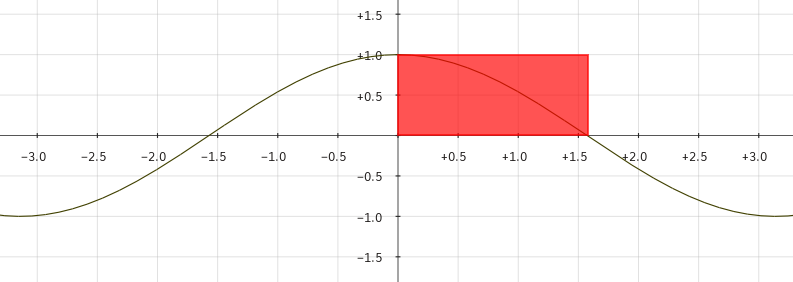
\includegraphics[width=0.8\textwidth]{img/coseno.png}
\caption{Comportamiento de la función $\cos$. En rojo la región que involucra los resutlados de la función de similitud}
\label{bus:img-coseno}
\end{figure}
El dominio de la función de similitud son los vectores normalizados con todas sus componentes mayores o iguales a 0.\\
\begin{figure}[H]
\centering
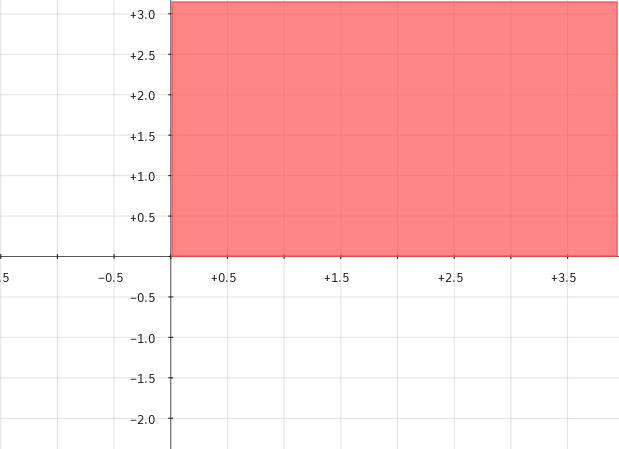
\includegraphics[width=0.4\textwidth]{img/planoCartesiano.png}
\caption{Plano cartesiano. En rojo al cuadrante al que pertenecen los vectores}
\label{bus:img-planoCartesiano}
\end{figure}
Del dominio de la función se obtiene que los ángulos que se forman se encuentran limitados entre $0$\textdegree y $90$\textdegree, 
o lo que es lo mismo $0$ y $\frac{\pi}{2}$. 
De lo anterior se obtien que:
$$0\leq \cos(\hat{\theta}) \leq 1$$
En el intervalo $[0, 1]$ la función $\cos$ es decreciente. Por lo que se definie la función de similitud como el $\cos$ del ángulo que forman de dos vectores. 
De esta manera los vectores tengan un ángulo cercano a $0$\textdegree son más similares. 

\section{Resolución}
Encontrar una solución al problema planteado es reducible 

El algoritmo que se utilizó para obtener las soluciones es \texttt{Produce-and-Choose}, cuenta con 
dos fases.
En la primer fase se generan cierta cantidad de bundles, e la fase siguiente se seleccionan los 
bundles que serán parte de la solución.\\
A continuación se explican los algoritmos utilizados para cada fase.
\section{Generación de bundles}
Dado un conjunto de papers el objetivo es generar clusters en los cuales los papers suficientemente 
similares pertenezcan al mismo cluster y en cluster distintos los disímiles. Cuanto mayor es la 
similitud en el cluster (intra) y mayor la diferencia entre los cluster (inter) es mejor la 
clusterización.\\
Definir como se constituye un cluster es complejo. Por ejemplo para los 20 puntos que se muestran a 
continuación existen tres (o más) formas de clusterizar que son validas. Entonces la mejor 
definición depende del tipo de dato y del resultado esperado.

\begin{figure}[H]
  \centering
    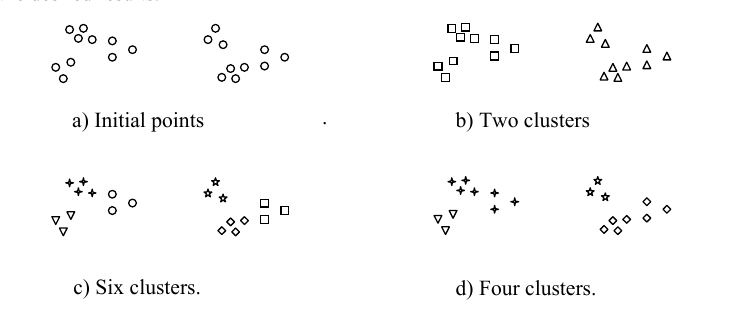
\includegraphics[width=0.8\textwidth]{img/howToCluster.png}
  \caption{Agregar descripcion}
  \label{res:img-howToCluster}
\end{figure}

En la clusterización para Composite Retrival, la definición es generar cluster máximizando el costo que esta acotado por el budget.
Ya que lo esperado es obtener cluster que utilicen el máximo del presupuesto.\\

El problema de la clusterización es NP-hard (agregar ref, explicar problema de clusterizacion),
por lo que se utilizaron dos técnicas ya conocidas para aproximarse a una solución.\\
La principal diferencia entre las estrategias de clusterización es entre la jerárquica y de 
partición.\\
La primer técnica produce un árbol de particiones, la raíz es un cluster que contiene todos los items
y las hojas son clusters con un único ítem. Cada nivel intermedio, puede ser visto, como la 
combinación entre dos clusters del nivel inferior inmediato. Mientras que la segunda genera solo un 
nivel de las particiones de los items de una vez.\\ 
Se implementaron las dos técnicas para la clusterización jerárquica con el algoritmo
Hierarchical clustering y la de partición con Bundles One-By-One.\\

\subsection{Bundles One-By-One}
El método \texttt{BOBO-x} esta inspirado en k-nn. Consiste en cada paso seleccionar, de manera azarosa, un item del conjunto de pivotes (en el inicio este conjunto contiente todos los items),
con el que se genera un bundle valido a al rededor de este. En el caso de que el intra del bundle sea bueno se agrga al conjunto de candidatos de bundle.
La iteración finaliza cuando se generan la cantidad de candidatos definidos en el parámetro $x$ o cuando el conjunto de bundles es vacío. El caso de que $x$ sea 'Ex' todos los 
items son pivotes.\\
Para generar el bundle a partir del pivote, se realiza de manera golosa de eligiendo en cada iteración el item que
máximiza el intra y que cumple con las resticciones.\\
\subsection{Hierarchical clustering}
La heurística Hierarchical clustering \texttt{HAC} comienza con tantos clusters como cantidad de elementos, cada uno está 
conformado por un solo ítem y en cada paso se unen los dos clusters más cercanos que respetan las restricciones. 
Para ello se define la función de distancia para los items $u$ y $v$ como:\\
\begin{equation}
d_{1}(u,v) = 1 - s(u, v)
\end{equation}

Con la función de distancia $d_{1}$ en la clusterización se generan los cluster lo más cohesivos posibles,
En la figura 1 se observa que el algoritmo selecciona los items más cercanos. En las búsquedas que 
se realizan en ``Composite ...''\cite{compositeRetrival} se tiene el parámetro $\gamma$ que indica 
que tipo de resultado es el esperado. 

\begin{figure}[H]
  \centering
    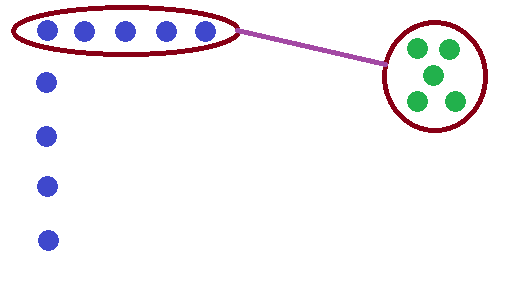
\includegraphics[width=0.3\textwidth]{img/cluster2.png}
  \caption{Selección de bundles usando $d_{1}$}
  \label{res:img-usingEfficientHAC}
\end{figure}

En caso de que el $\gamma$ sea pequeño, la 
clusterización esperada para la misma instancia es la que se visualiza en la imágen 2, clusters no 
tan cohesivos pero más variados. Por lo que se define una función de distancia que considera el 
$\gamma$.\\
\begin{equation}
d2(u,v) = 1 - FO(\{u\} \cup \{v\})
\end{equation}
Donde $FO$ es la función definida en \eqref{eq:fnObj} \\

\begin{figure}[H]
  \centering
    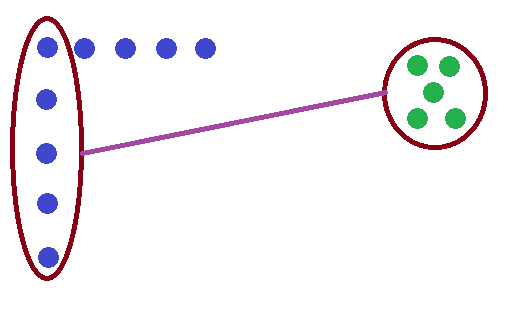
\includegraphics[width=0.3\textwidth]{img/cluster1.png}
  \caption{Selección de bundles usando $d_{2}$}
  \label{res:img-usingSingleHAC}
\end{figure}

Para la distancia $d_{1}$ se implementó el algoritmo \texttt{EfficientHAC} que es tiene una 
complejidad $\mathcal{O}(n^{2})$, mientras que para $d_{2}$ el algoritmo es \texttt{SingleHAC} que 
la complejidad es $\mathcal{O}(n^{2} * \ln{n})$. Según se demostró en el capítulo 17 de 
\cite{informationRetrival}


\section{Selección de bundles}
Al finalizar la producción de bundles, se deben seleccionar los $k$ bundles para la solución.
El problema de seleccionar los bundles que maximizan la función objetivo, se traduce en 
encontrar en el grafo G el k-subgrafo de mayor peso de nodos y aristas.

Se implementó el algoritmo que propone ``Composite ...''\cite{compositeRetrival} que transforma el 
grafo G en el grafo G', con los mismos nodos y aristas, redefiniendo el peso de las aristas con la 
función:\\

\begin{equation}
\omega_{1}(u,v) = \dfrac{\gamma}{2( k - 1)} (\omega(u) + \omega(v)) + (1 - \gamma)\psi(u,v) 
\end{equation}

(aca va el algoritmo)\\

En la función $\omega_{1}(u,v)$ el valor de la función $\psi(u,v)$  es considerablemente menor al de
$\omega(u) + \omega(v)$, (en el intra se suma los ejes de todos los nodos, el inter es el máximo entre los items)
implica que $\gamma$ no cumple con el objetivo de balancear entre una solución cohesiva y una variada.
Para esto se funciones $\omega$ alternativas.\\

Con $\omega_{2}(u,v,w,y)$ la búsqueda se realiza con la combinación de cuatro nodos, por lo que el orden de complejidad
aumenta a ...

\begin{equation}
\begin{split}
\omega_{2}(u,v,w,y) &= \dfrac{\gamma}{2( k - 1)} (\omega(u) + \omega(v) + \omega(w) + \omega(y)) \\
&+ (1 - \gamma)(\psi(u,v) + \psi(u,w) + \psi(u,y)  + \psi(v,w) + \psi(v,y) + \psi(w,y))
\end{split}
\end{equation}

La función $\omega_{3}(u, k)$ recibe $u$ el conjunto de clusters seleccionados hasta el momento 
y $k$ que es la cantidad de clusters para la solución. Con $k$ y el tamaño de $u$ se calcula el 
coeficiente con el propósito en que en cada paso se pondere el inter y el intra. Para eso se multiplica
con coeficientes cada parte de la función. Con esto se mantiene la relación de inter e intra durante la selección de bundles

\begin{equation}
\begin{split}
\omega_{3}(u,k) &= \dfrac{k}{u.size} * (\gamma \sum_{v \in U}(w(v))) \\
&+ \dfrac{(k * (k-1))}{2} * \dfrac{2}{(u.size() * (u.size() - 1))} * 1 - \gamma \sum_{v,w \in U}(\psi(v,w))
\end{split}
\end{equation}

\begin{algorithm}[H]
\begin{algorithmic}[1]
\REQUIRE $produced:Vector<SnowFlake>, numRequested:Integer$
\ENSURE $selected:Vector<SnowFlake>$.
\STATE $selected:Vector<SnowFlake> \leftarrow []$
\STATE $originalSize:Integer \leftarrow produced.size$
\WHILE {$selected.size < numRequested\ AND\ selected.size < originalSize$}
\STATE $selectedTemp \leftarrow selected$
\STATE $(candidateOne, candidateTwo) \leftarrow (i, j)\ where$ \\ 
$\displaystyle\max_{i \neq j} (FO(selectedTemp.push(produced_{i} \cup produced_{j})))$
\STATE $produced.erase(i)$
\STATE $produced.erase(j)$
\STATE $selected.push(candidateOne)$
\STATE $selected.push(candidateTwo)$
\ENDWHILE
\RETURN $selected$
\end{algorithmic}
\caption{Selección de bundles de a pares}\label{alg:algSelTuple}
\end{algorithm}
\subsection{Selección proporcional}
Además como tercera opción de selección se implementó un algoritmo proporcional que en cada paso se 
ponderan los resultados de la función que calcula el intra y el inter restante, intentando 
\textquotedblleft adivinar\textquotedblright  el valor de las próximas iteraciones y de esta manera 
dar más importancia en los primeras iteraciones al valor del inter.
\begin{algorithm}[H]
\begin{algorithmic}[1]
\REQUIRE $produced:Vector<SnowFlake>, numRequested:Integer$
\ENSURE $selected:Vector<SnowFlake>$
\STATE $w(u) = \dfrac{k}{u.size} * (\gamma \sum_{v \in U}(w(v))) + \dfrac{(k * (k-1))}{2} * \dfrac{2}{(u.size() * (u.size() - 1))} * 1 - \gamma \sum_{v,w \in U}(\psi(v,w))$
\STATE $available \leftarrow produced$
\STATE $selected \leftarrow []$
\WHILE {$selected.size < numRequested\ AND\ selected.size < produced.size$}
\STATE $candidate \leftarrow max_{i}$
\ENDWHILE
\RETURN $selected$
\end{algorithmic}
\caption{Selección de bundles proporcional}\label{alg:algSelProp}
\end{algorithm}

\section{Modificación de PAC para búsquedas específicas}
Para la obtención de la solución se modificó la producción de bundles como así también la 
selección de los mismos (Produce and Choose). \\
En la producción de bundles en el algoritmo jerárquico, se utilizó la similitud del perfil 
específico con los papers en cada paso que intenta unificar dos clusters. A diferencia del cálculo 
original que la compatibilidad de dos nodos esta dada por su distancia previamente obtenida, en 
este nuevo caso se agrega a ese resultado la compatibilidad de cada uno de ellos con el perfil 
específico. \\
Para la producción del algoritmo BOBO, se agregó junto al pivote en todos los clusters. \\
Para la selección de los bundles que formarán parte de la solución, a cada cluster se le 
calculo el valor intra también se tuvo en cuenta la similitud de todos los elementos con el perfil  
específico, de esta manera a los clusters que contenían papers con los mismos tópicos que el del 
vector especifico se le dio mayor peso.

\section{Heurística golosa para la obtención de una solución}
En todas los algoritmos previos se centraron en, primero construir buenos bundles maximizando solo 
el valor propio de cada bundle, o sea, el valor inter bundle. Una vez generado los suficientes 
\textquotedblleft buenos\textquotedblright  para luego seleccionar dependiendo de la 
estrategia elegida la solución final, ahora si, maximizando la función objetivo propuesta 
originalmente.\\
Para este heurística golosa propusimos ir construyendo los bundles finales teniendo en cuenta en 
cada paso la función objetivo, esto es, en cada paso cuando se intenta agregar un nuevo elemento a 
un bundle se calcula su valor total de la función y se evalúa en que bundle conviene agregarlo. 
Esto se repite para todos los items, haciendo que cuando tengo que agregar un nuevo ítem a la 
solución ya calculé para todos los items que no se encuentran en la solución en que bundle conviene 
agregarlo y cual es el valor de la función en ese caso, quedándonos siempre con el mejor valor 
posible.
\begin{algorithm}[H]
\begin{algorithmic}[1]
\REQUIRE $numOfSnowFlakes:Integer$
\ENSURE $selected:Vector<SnowFlake>$
\STATE $selected_{i}:Vector<SnowFlake> \leftarrow \emptyset_{0\leq i<numOfSnowFlakes}$
\STATE $isComplete:Bool \leftarrow False$
\STATE $elements:Set<Element> \leftarrow ElementsOfTheProblem$
\WHILE {$isComplete == False$}
\STATE $bestScore:Double \leftarrow -\infty$
\STATE $bestElement:Element \leftarrow \varnothing$
\STATE $bestBundle:SnowFlake \leftarrow \varnothing$
\FOR {$elem:Element \in elements$}
\FOR {$bundle:SnowFlake \in selected$}
\IF {$isValidBundle(bundle \cup \{elem\}) == True$}
\STATE $score:Double \leftarrow FO(selected.replace(bundle, bundle \cup \{elem\}))$
\IF {$score > bestScore$}
\STATE $bestScore \leftarrow score$
\STATE $bestBundle \leftarrow bundle$
\STATE $bestElement \leftarrow elem$
\ENDIF
\ENDIF
\ENDFOR
\ENDFOR
\STATE $selected \leftarrow selected.replace(bundle, bundle \cup \{elem\})$
\STATE $elements.erase(elem)$
\STATE $isComplete \leftarrow bestElement == \varnothing$
\ENDWHILE
\RETURN $selected$
\end{algorithmic}
\caption{Algoritmo heurística golosa}\label{alg:algHeuGol}
\end{algorithm}

\chapter{Resultados}
\section{Comparando soluciones}
Para comparar la calidad de las distintas soluciones, además del valor objetivo se compara con 
la cantidad de elementos iguales en toda la solución y la cantidad igual de elementos para cada 
bundle. De esta manera se observa que tan \textquotedblleft parecidas\textquotedblright son las 
soluciones y con más detalle que tan \textquotedblleft parecidos\textquotedblright son los bundles. 
Entre los diferentes algoritmos buscamos la cantidad de elementos iguales en cada una de las 
soluciones y también la cantidad de elementos iguales por bundle.
\section{Papers}
Originalmente la base de datos contenía unos 7777 papers, de los cuáles se tuvo que hacer una 
depuración, ya que había papers que no tenían ningún autor asociado o perfil creado. Luego de la 
depuración obtuvimos 4937 que cumplen los requisitos para la búsqueda de las soluciones.\\
Se genraron soluciones con las siguientes características:\\
\Solucion
{}
{simple}
{\texttt{SingleHAC}, \texttt{EfficientHAC} y \texttt{Greedy}}
{$\in$ $(0,1; 0,3; 0,5; 0,7; 0,9)$}
{10}
{5}
Como primera observación podemos ver la cantidad de bundles que se generan para cada algoritmo de 
producción:\\
\begin{table}[h]
  \centering
  \resizebox{0.5\textwidth}{!} {
    \begin{tabular}{|lc|}
    \hline
    Algoritmo & Bundles Generados \\
    \hline
    SingleHAC & $2378$ \\
    EfficientHAC & $2378$ \\
    Greedy & $10$ \\
    \hline
    \end{tabular}
  }
    \caption {Cantidad de bundles generados antes de la selección final}
\end{table}

En los siguientes gráficos se visualiza los resultados obtenidos para $\gamma$ 0.1 y 0.9. Cada 
nodo representa un bundle y los ejes el valor de la similitud entre cada uno de ellos. La línea más 
gruesa indica un mayor grado de similitud. En cuanto a los vértices al acercarse al azul el valor 
de la intra es menor y al rojo mayor.

\begin{figure}[H]
  \centering
    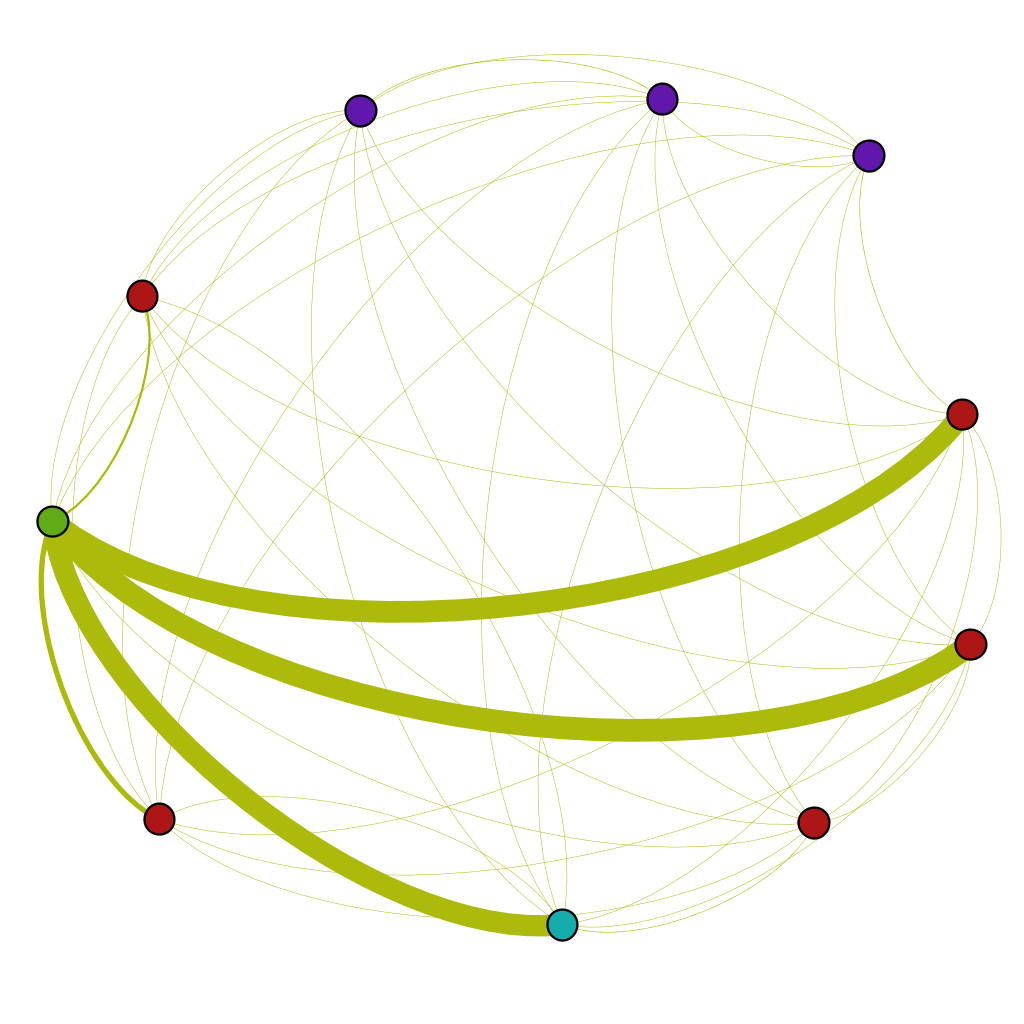
\includegraphics[width=0.5\textwidth]{resultados/papers/intra_inter/hac01.png}
  \caption{Relación entre bundles para $\gamma$ = $0.1$ y algoritmo SingleHAC}
  \label{res:img-papers-gamma01-hac}
\end{figure}

\begin{figure}[H]
  \centering
    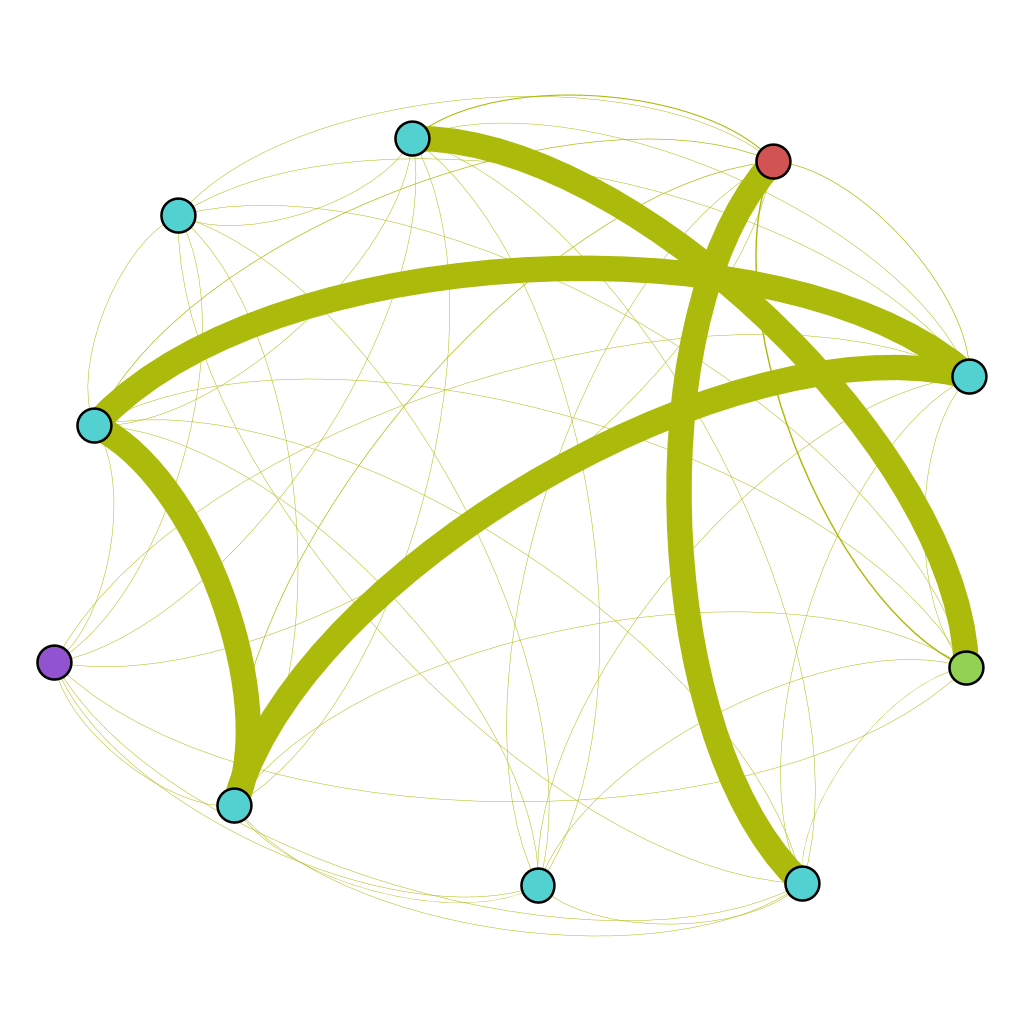
\includegraphics[width=0.5\textwidth]{resultados/papers/intra_inter/hac09.png}
  \caption{Relación entre bundles para $\gamma$ = $0.9$ y algoritmo SingleHAC}
  \label{res:img-papers-gamma09-hac}
\end{figure}

\begin{figure}[H]
  \centering
    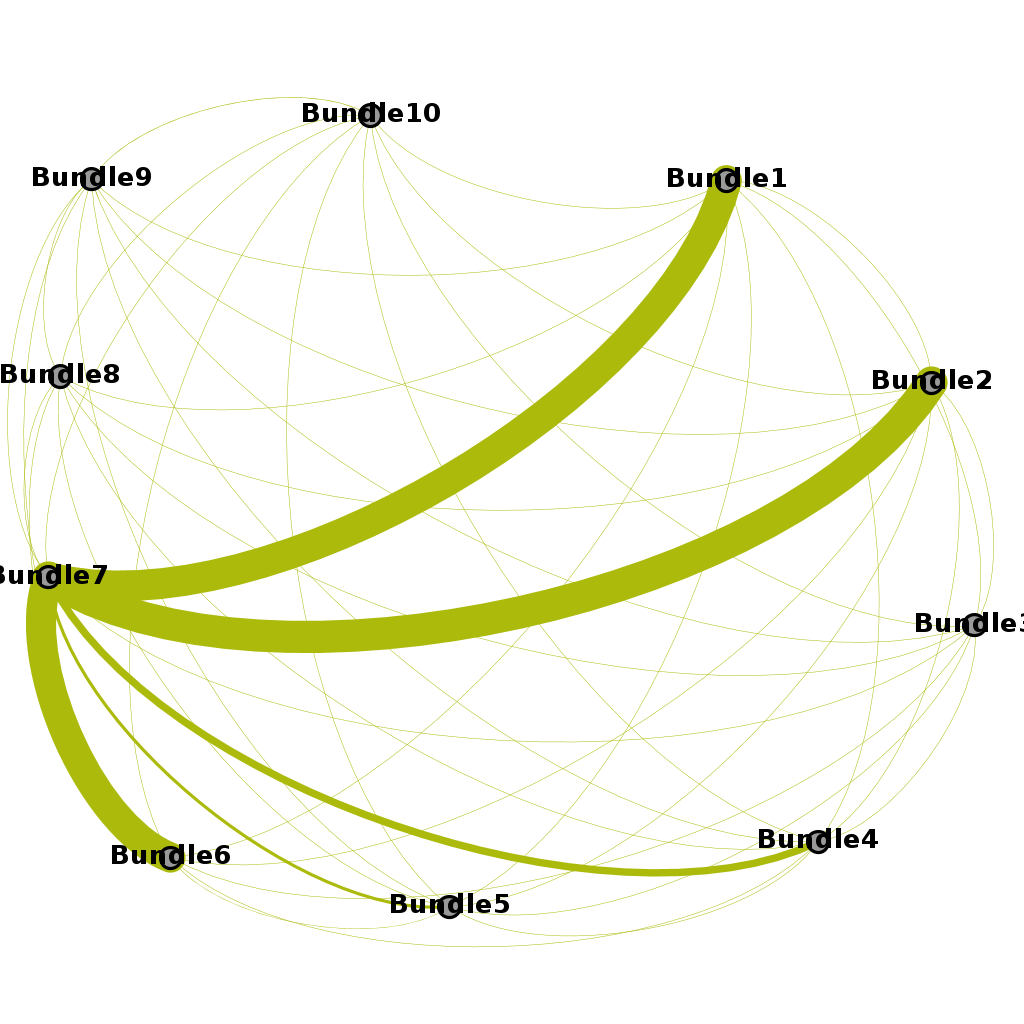
\includegraphics[width=0.5\textwidth]{resultados/papers/intra_inter/effhac01.png}
  \caption{Relación entre bundles para $\gamma$ = $0.1$ y algoritmo EfficientHAC}
  \label{res:img-papers-gamma01-effhac}
\end{figure}

\begin{figure}[H]
  \centering
    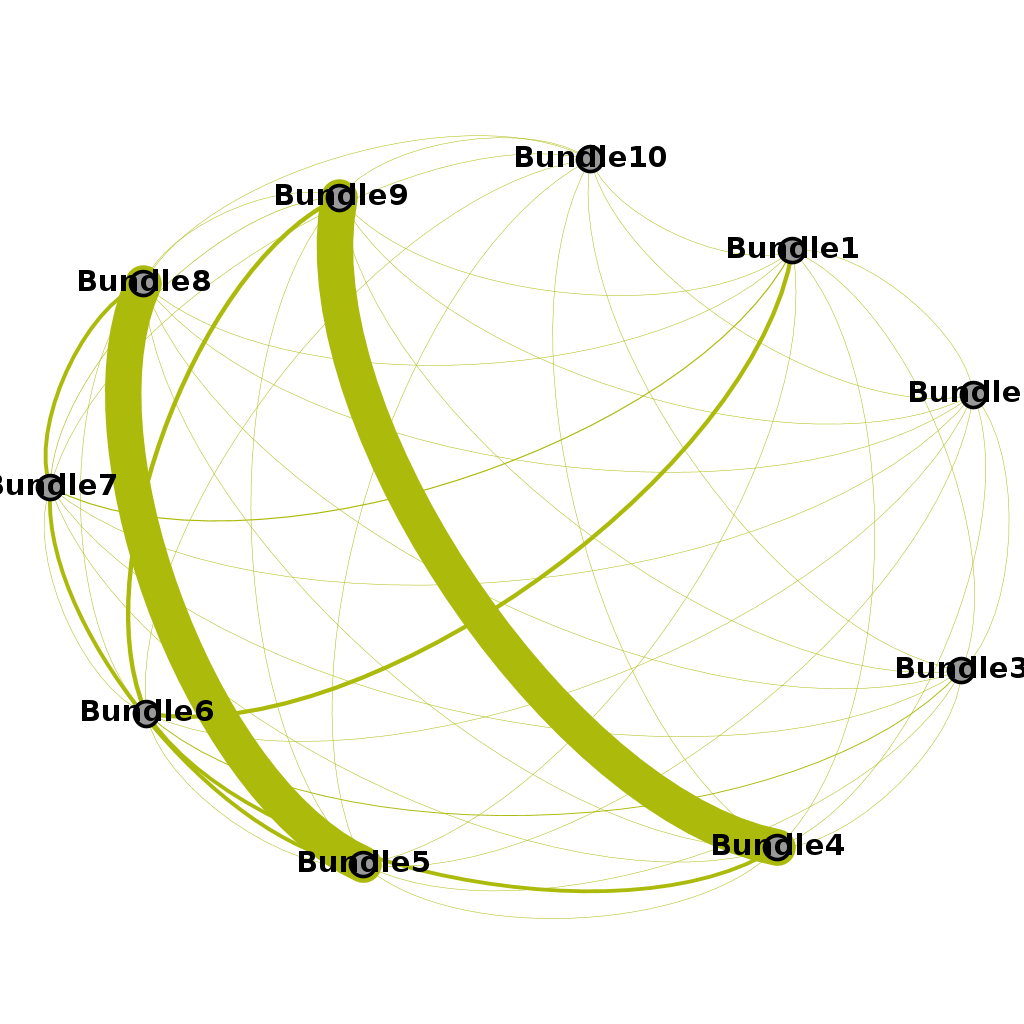
\includegraphics[width=0.5\textwidth]{resultados/papers/intra_inter/effhac09.png}
  \caption{Relación entre bundles para $\gamma$ = $0.9$ y algoritmo EfficientHAC}
  \label{res:img-papers-gamma09-effhac}
\end{figure}

\begin{figure}[H]
  \centering
    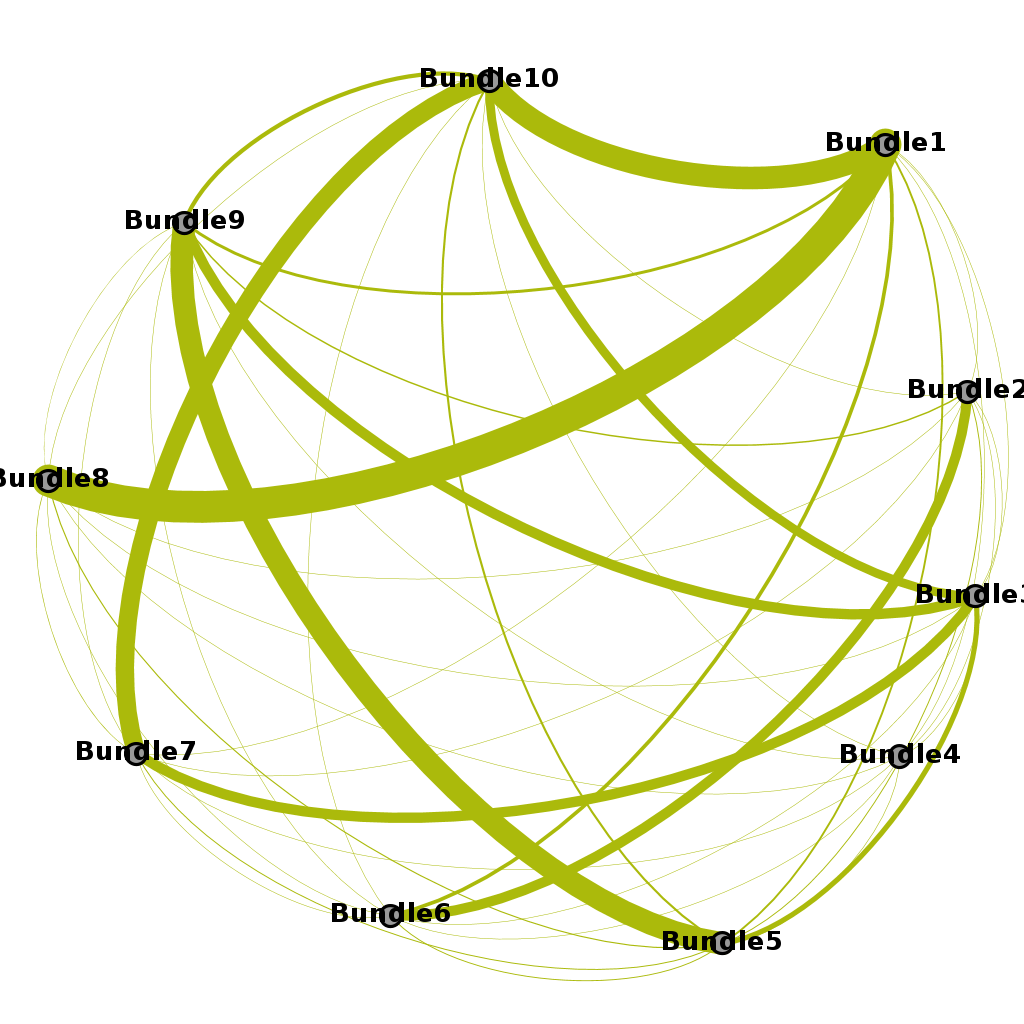
\includegraphics[width=0.5\textwidth]{resultados/papers/intra_inter/greedy01.png}
  \caption{Relación entre bundles para $\gamma$ = $0.1$ y algoritmo Greedy}
  \label{res:img-papers-gamma01-greedy}
\end{figure}

\begin{figure}[H]
  \centering
    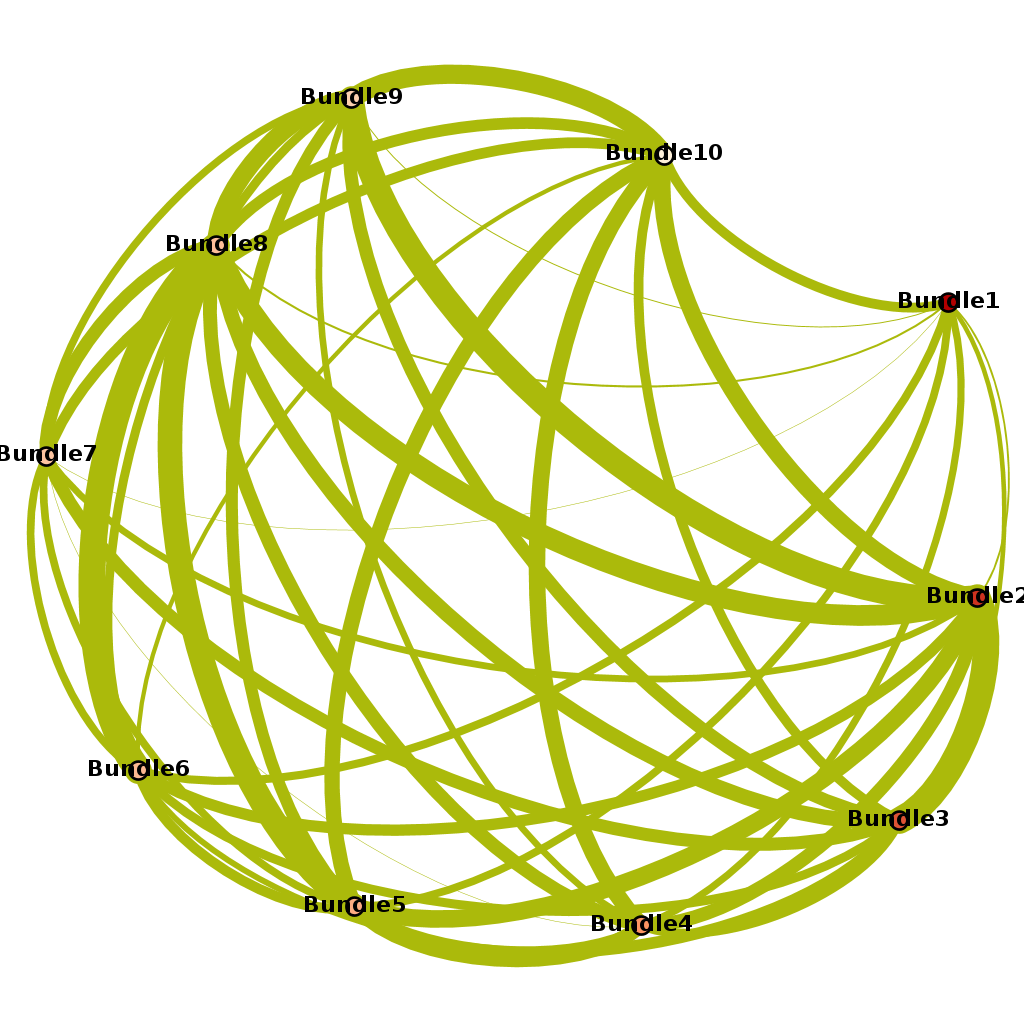
\includegraphics[width=0.5\textwidth]{resultados/papers/intra_inter/greedy09.png}
  \caption{Relación entre bundles para $\gamma$ = $0.9$ y algoritmo Greedy}
  \label{res:img-papers-gamma09-greedy}
\end{figure}

\section{Autores}
Se genraron soluciones con las siguientes características:\\
\Solucion
{}
{simple y proporcional}
{\texttt{SingleHAC}, \texttt{EfficientHAC} y \texttt{Greedy}}
{$\in$ $(0,1; 0,3; 0,5; 0,7; 0,9)$}
{10}
{5}

En los siguientes gráficos se visualiza los resultados obtenidos para $\gamma$ 0.1 y 0.9. Cada 
nodo representa un bundle y los ejes el valor de la similitud entre cada uno de ellos. La línea más 
gruesa indica un mayor grado de similitud. En cuanto a los vértices al acercarse al azul el valor 
de la intra es menor y al rojo mayor.

\begin{figure}[H]
  \centering
    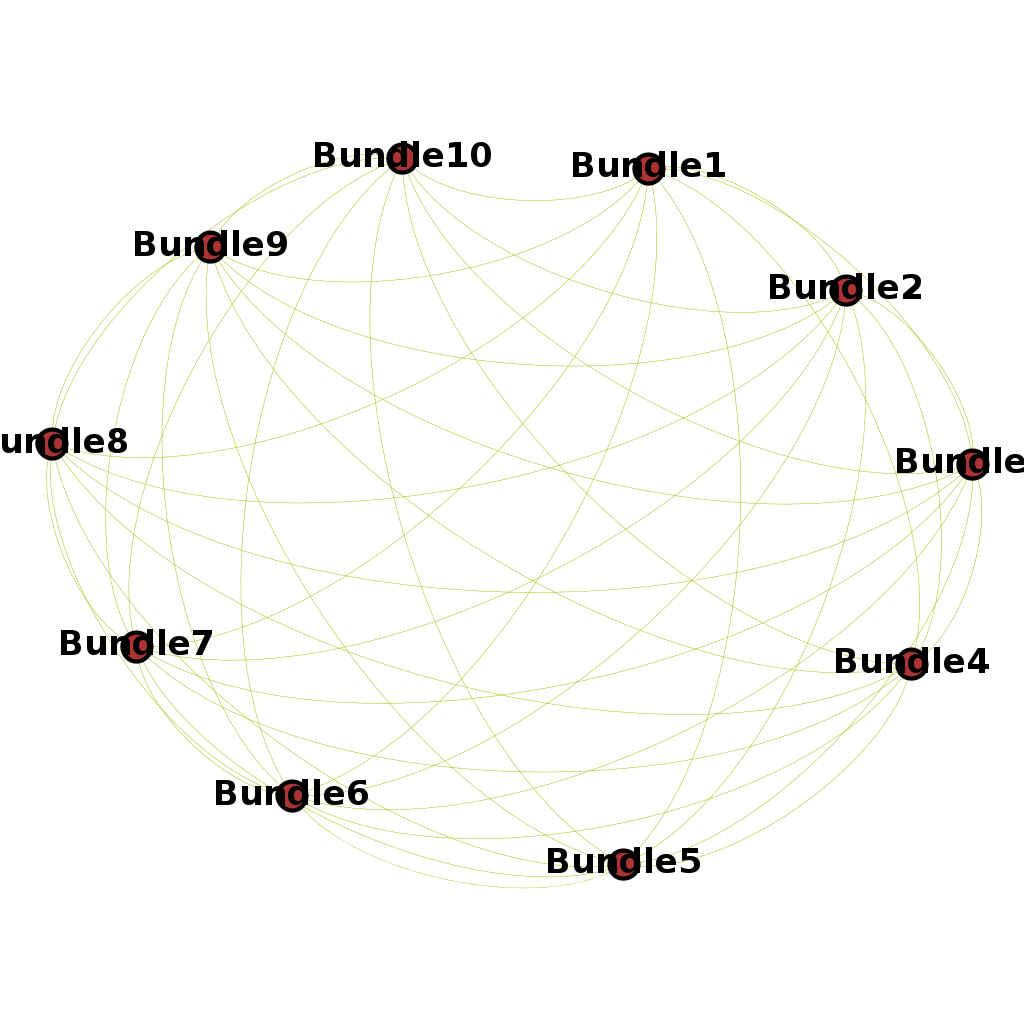
\includegraphics[width=0.5\textwidth]{resultados/authors/intra_inter/hac01.png}
  \caption{Relación entre bundles para $\gamma$ = $0.1$ y algoritmo SingleHAC, selección simple}
  \label{res:img-authors-gamma01-hac}
\end{figure}

\begin{figure}[H]
  \centering
    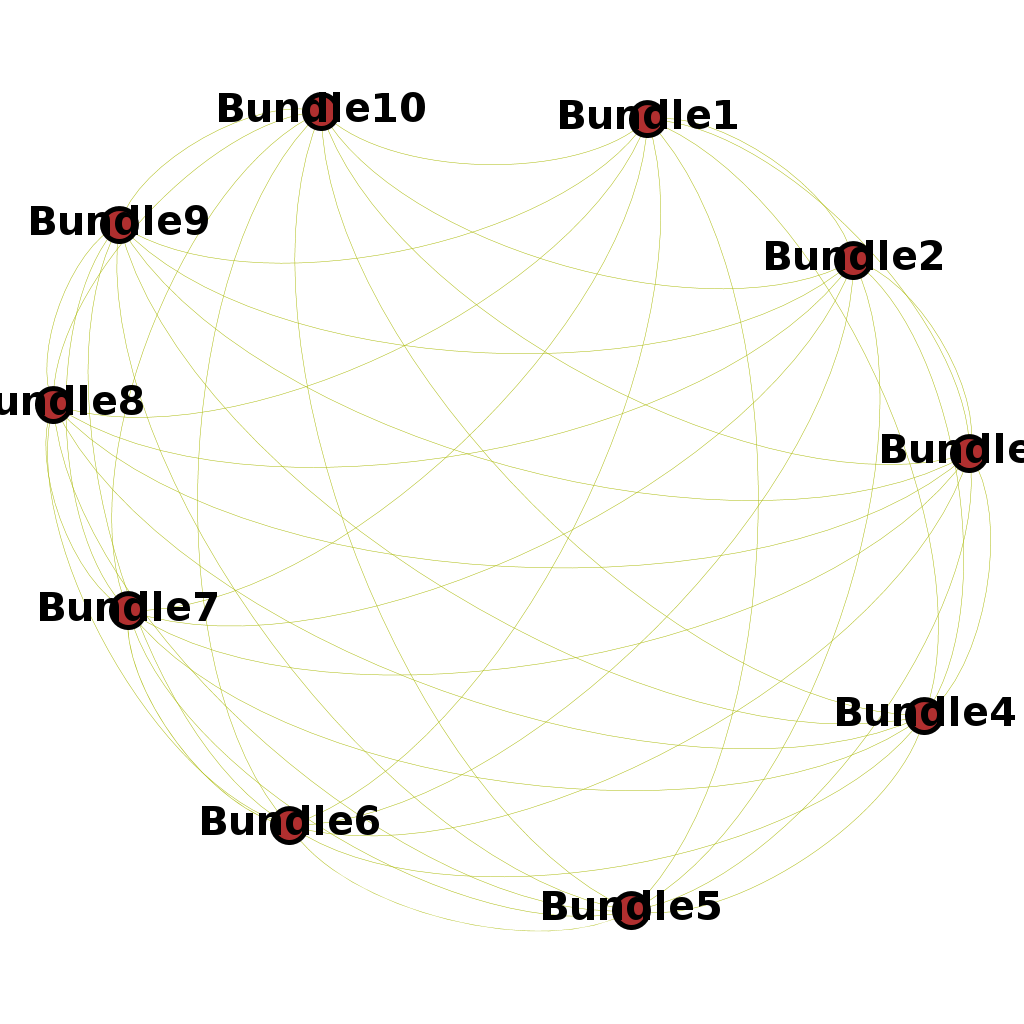
\includegraphics[width=0.5\textwidth]{resultados/authors/intra_inter/hac09.png}
  \caption{Relación entre bundles para $\gamma$ = $0.9$ y algoritmo SingleHAC, selección simple}
  \label{res:img-authors-gamma09-hac}
\end{figure}

\begin{figure}[H]
  \centering
    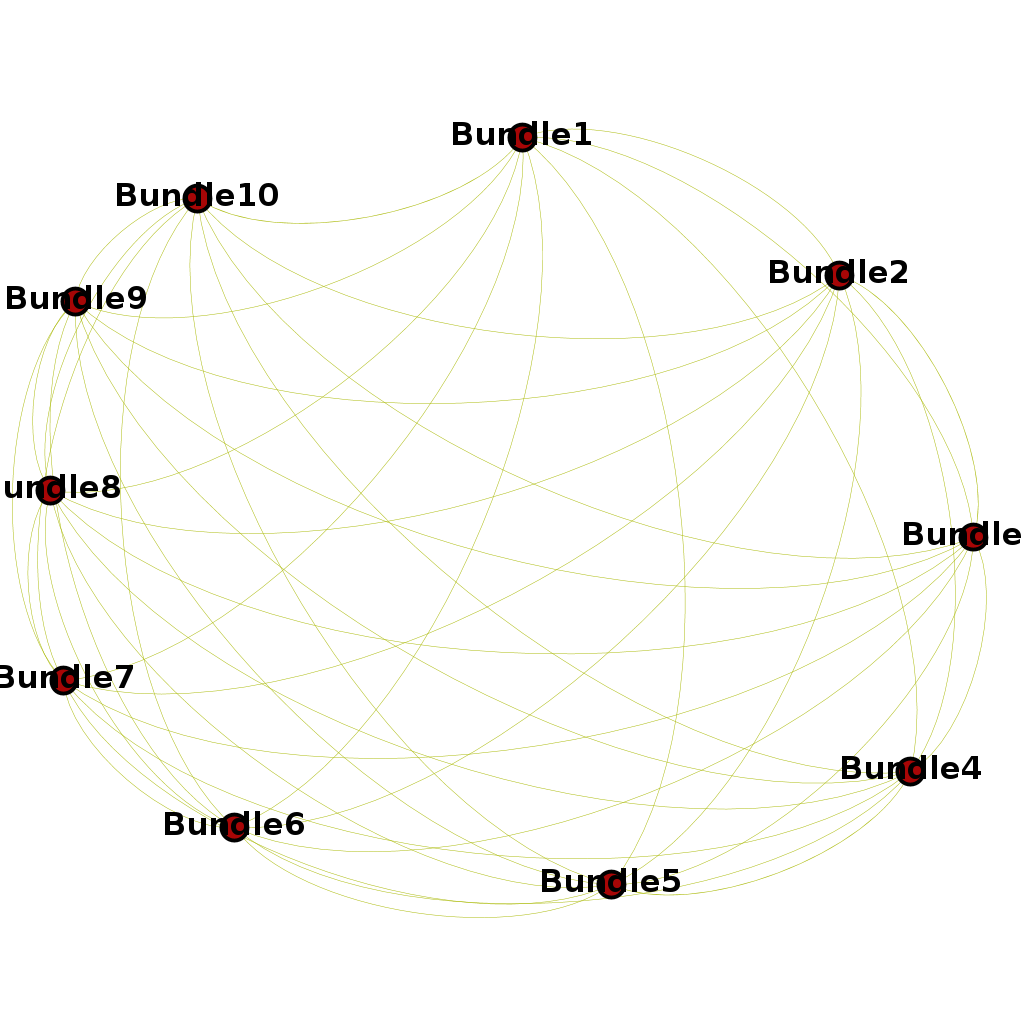
\includegraphics[width=0.5\textwidth]{resultados/authors/intra_inter/effhac01.png}
  \caption{Relación entre bundles para $\gamma$ = $0.1$ y algoritmo EfficientHAC, selección simple}
  \label{res:img-authors-gamma01-effhac}
\end{figure}

\begin{figure}[H]
  \centering
    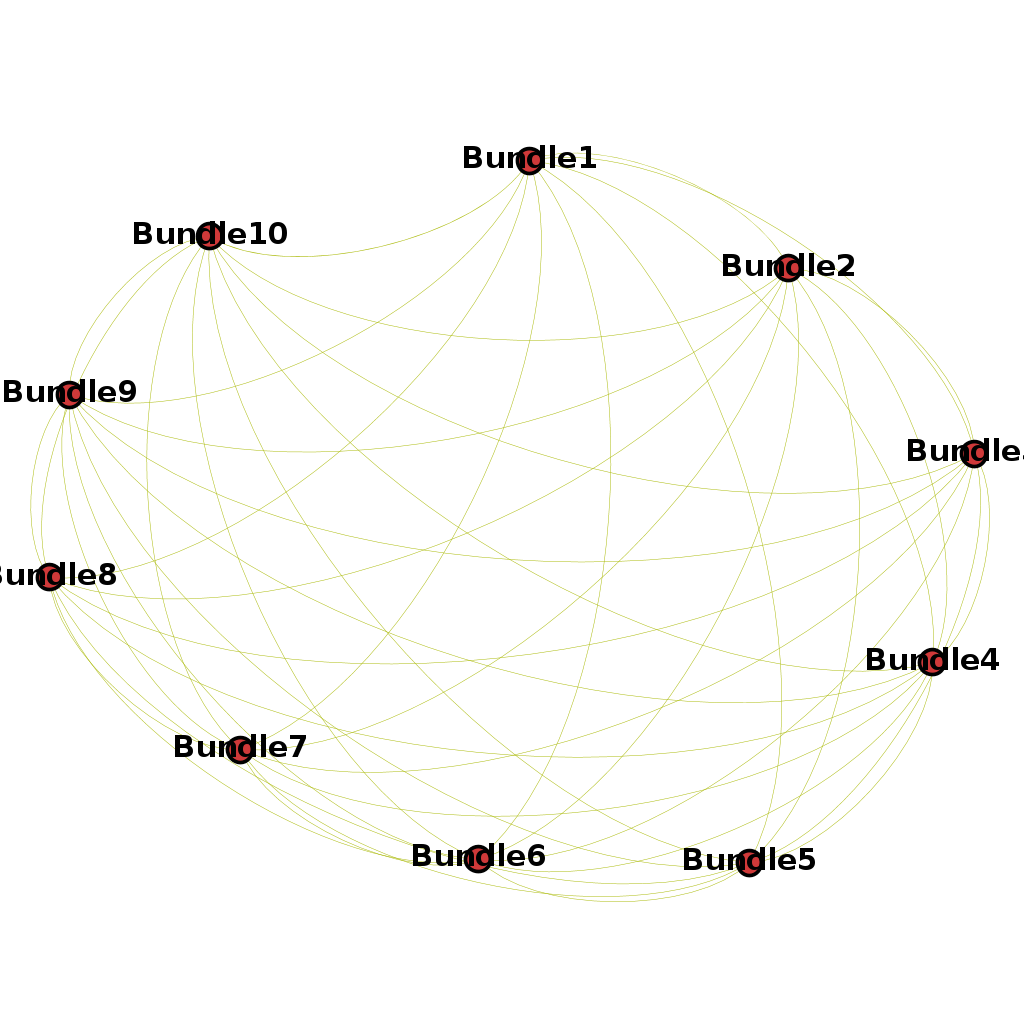
\includegraphics[width=0.5\textwidth]{resultados/authors/intra_inter/effhac09.png}
  \caption{Relación entre bundles para $\gamma$ = $0.9$ y algoritmo EfficientHAC, selección simple}
  \label{res:img-authors-gamma09-effhac}
\end{figure}

\begin{figure}[H]
  \centering
    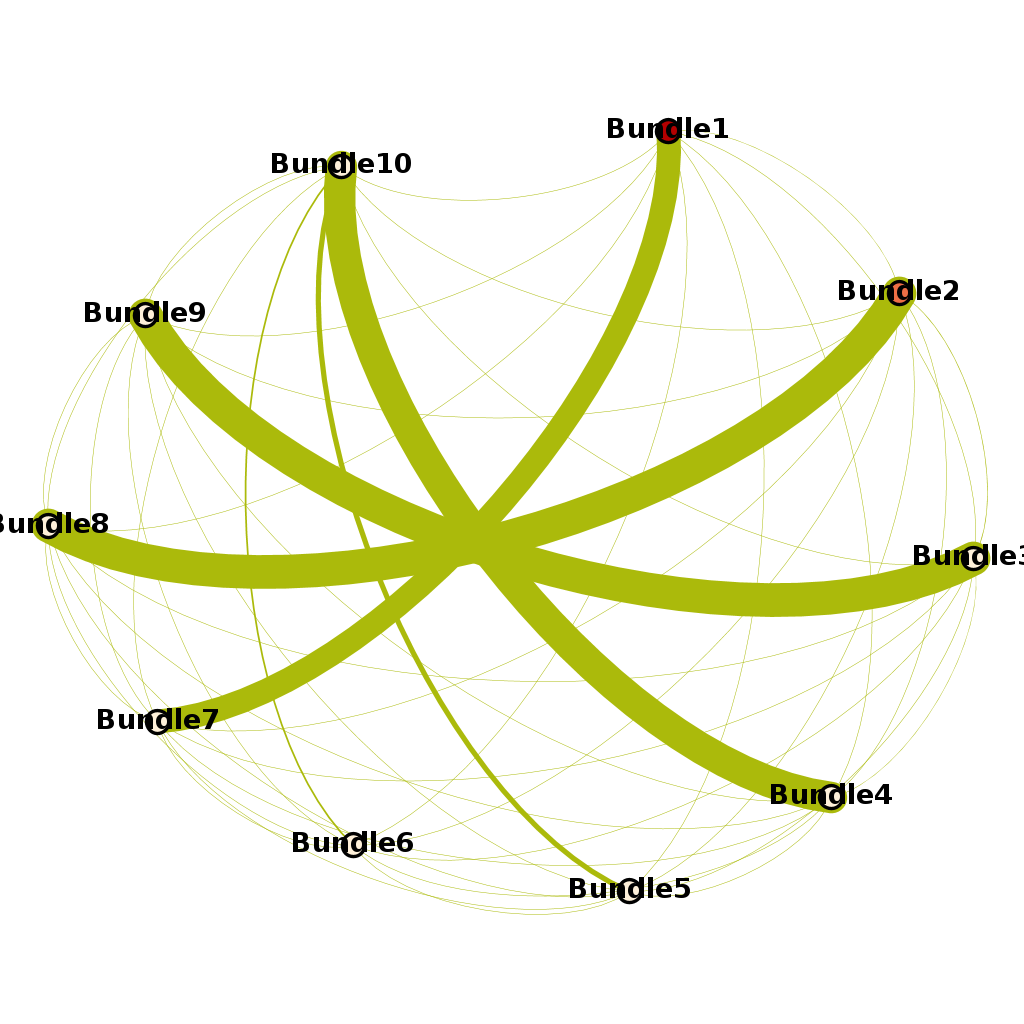
\includegraphics[width=0.5\textwidth]{resultados/authors/intra_inter/greedy01.png}
  \caption{Relación entre bundles para $\gamma$ = $0.1$ y algoritmo Greedy}
  \label{res:img-authors-gamma01-greedy}
\end{figure}

\begin{figure}[H]
  \centering
    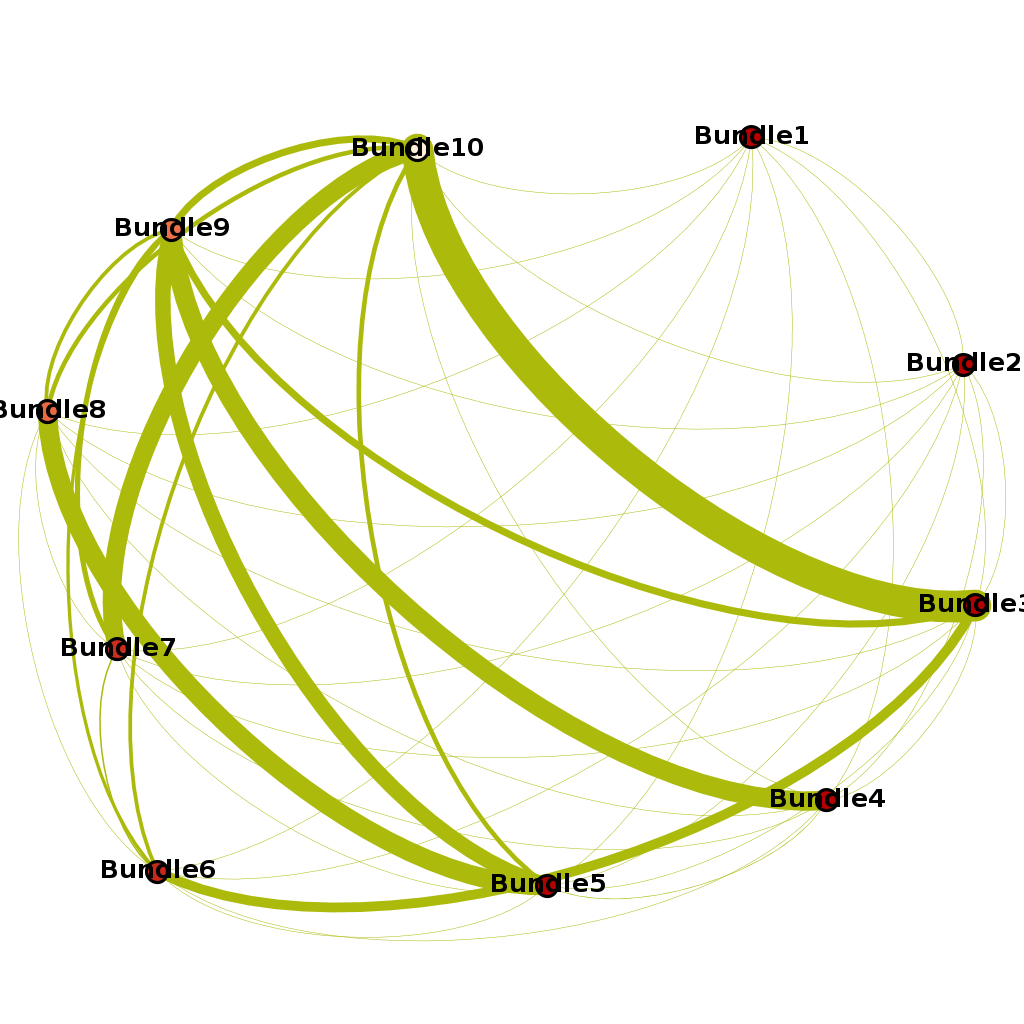
\includegraphics[width=0.5\textwidth]{resultados/authors/intra_inter/greedy09.png}
  \caption{Relación entre bundles para $\gamma$ = $0.9$ y algoritmo Greedy}
  \label{res:img-authors-gamma09-greedy}
\end{figure}

Tanto para las soluciones generadas por \texttt{SingleHAC} como por \texttt{EfficientHAC} y con 
cualquier estrategia de selección, todas las soluciones formaron los mismos bundles a pesar de la 
variación del parámetro $\gamma$. Esto se puede ver en los gráficos ya que todos los bundles 
tienen el mayor valor posible para la similitud intra y ningún bundle tiene relación con el 
resto.\\
En parte se debe a que existen $40000$ relaciones de similitud con valor uno. Con la 
heurística Produce and Choose, al momento de producir no se tiene en cuenta el $\gamma$ por lo tanto 
para todos los $\gamma$ en la etapa de producción se producen los mismos bundles.\\
Se realizaron otras búsquedas de soluciones, excluyendo a cinco de los autores que se encuentran 
presentes en todas las soluciones. Pero aún de esta manera en los nuevos resultados obtenidos se 
repite el mismo comportamiento que antes.\\
Además como veremos en \ref{conc:compDifAlgo} los resultados para las ejecuciones con los 
algoritmos jerárquicos se encuentran en los óptimos.
%Por otro lado todas las soluciones generadas por el algoritmo \texttt{HAC} prácticamente no 
%comparten bundles similares con las demás soluciones, ni siquiera autores similares en toda la 
%solución.

\section{Búsqueda con perfil específico}
En una primera aproximación para realizar esta búsqueda solo se modifico la generación de bundles, 
lo cuál, si bien genero resultados diferentes al algoritmo original, no se veía reflejado en los 
resultados las temáticas de los bundles con la elegida para la búsqueda. \\
A partir de ello se decidió modificar también la selección de los bundles para intentar obtener 
bundles relevantes con el perfil elegido. \\
A continuación mostramos la temáticas obtenidas para una búsqueda con un perfil específico de 
ALGORITHM = 50 \%, DISTRIBUTED SYSTEMS = 25 \% y KNOWLEDGE ENGINEERING = 25 \% para la ejecución 
del algoritmo jerárquico con $\gamma$ = 0.1 y $\gamma$ = 0.9.
\begin{figure}[H]
  \centering
    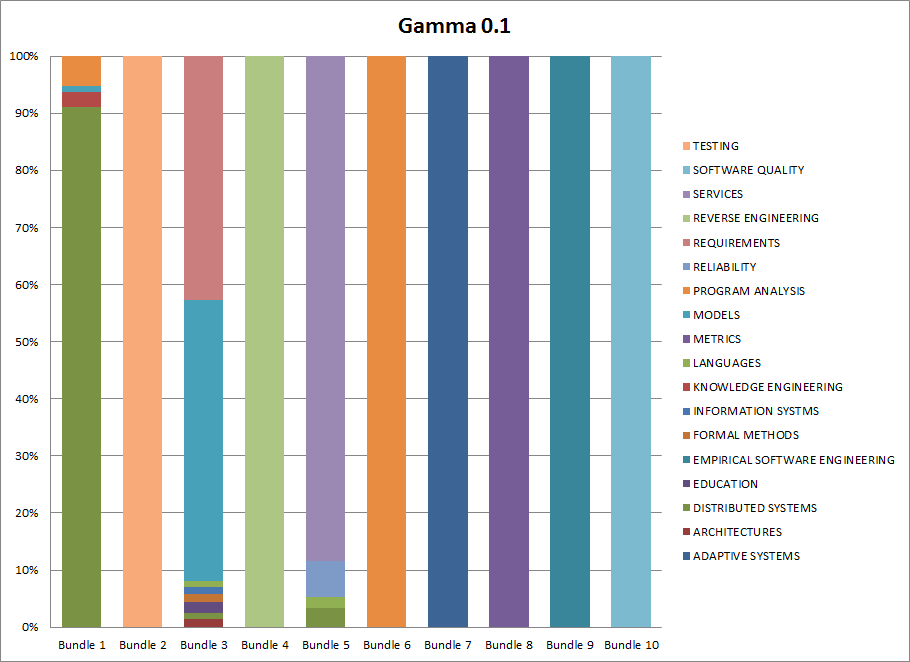
\includegraphics[width=\textwidth]{resultados/papers/intra_inter/grafico_gamm01.png}
  \caption{$\gamma$ = 0.1}
  \label{res:img-gamma01-especifico}
\end{figure}

\begin{figure}[H]
  \centering
    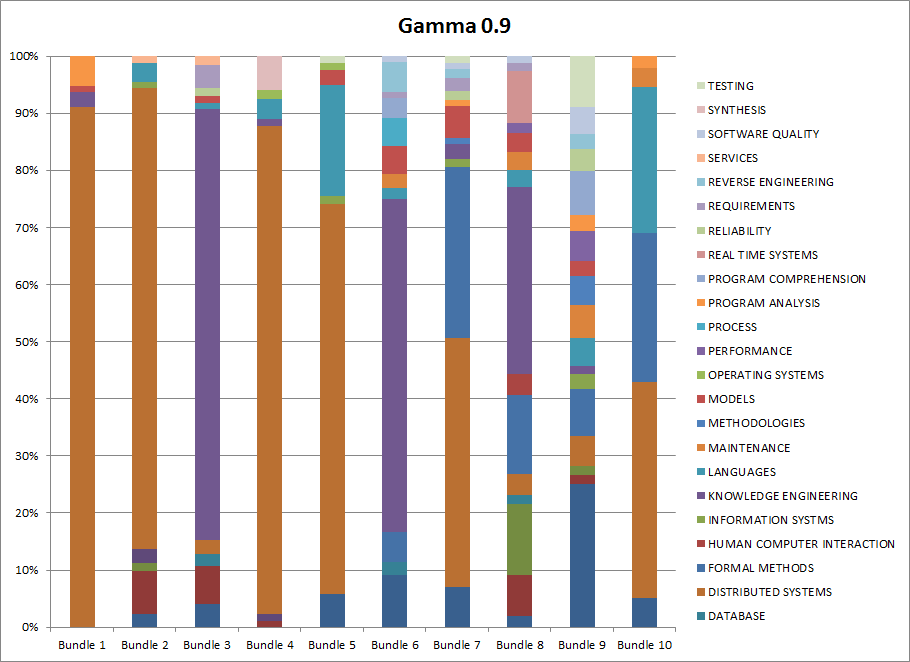
\includegraphics[width=\textwidth]{resultados/papers/intra_inter/grafico_gamm09.png}
  \caption{$\gamma$ = 0.9}
  \label{res:img-gamma09-especifico}
\end{figure}
\chapter{Conclusiones}
\section{Comparaciones entre los diferentes algoritmos}\label{conc:compDifAlgo}
\subsection{Papers}
Con los resultados obtenidos podemos hacer dos tipos de análisis y comparaciones, la primera y más 
clara es comparar entre los algoritmos \texttt{SingleHAC} y \texttt{EfficientHAC}, en la que 
observamos que para $\gamma$ bajos obtuvimos los mismos resultados, pero para $\gamma$ altos a 
partir de $0.7$ obtuvimos soluciones diferentes las cuáles tenían un valor con respecto a la 
función objetivo prácticamente iguales pero se obtuvieron mejores relaciones interbundles.\\
La otra comparación que surge es entre \texttt{EfficientHAC} y \texttt{Greedy} en el que se observa 
que para $\gamma$ las soluciones obtenidas son \textquotedblleft similarmente 
buenas\textquotedblright , dado que sus valores en términos de función objetivo están cercanos, 
pero a la vez observamos que la relación interbundles es mejor las soluciones de la implementación 
\texttt{Greedy}. En cambio para $\gamma$ altos, el valor de la función objetivo en la 
implementación \texttt{EfficientHAC} fue muy superior pero la relación interbundles en el algoritmo 
\texttt{Greedy} se ve que fue mejor, logrando soluciones mas interdependientes.

\section{Valores cercanos al óptimo}
Dada la función que se está intentando maximizar $$\displaystyle\sum_{1 \leq i \leq k} 
\displaystyle\sum_{u,v \in S_{i}} \gamma s(u,v)\ 
+\ \displaystyle\sum_{1 \leq i \leq j \leq k} (1-\gamma) (1 - \displaystyle\max_{u \in S_{1}, v 
\in S_{j}} s(u,v))$$ podemos hacer suposiciones para ver que tan lejos o cerca están de algunas de 
los valores óptimos según el $\gamma$.\\
Para las siguientes cotas supongamos escenarios ideales en el cuál la soluciones contiene bundles 
donde todos sus elementos tienen una similitud máxima (igual a 1) y los bundles entre si son 
completamente diferentes, o sea, la similitud entre cada bundle es 0. Con estas hipótesis podemos 
ver que la reemplazar la función por $$\displaystyle\sum_{1 \leq i \leq k} 
\displaystyle\sum_{u,v \in S_{i}} \gamma 1\ 
+\ \displaystyle\sum_{1 \leq i \leq j \leq k} (1-\gamma) (1 - \displaystyle\max_{u \in S_{1}, v 
\in S_{j}} 0)$$ que luego se transforma en $$\displaystyle\sum_{1 \leq i \leq k} 
\displaystyle\sum_{u,v \in S_{i}} \gamma 1\ 
+\ \displaystyle\sum_{1 \leq i \leq j \leq k} (1-\gamma) 1$$ como en nuestro caso $k\ =\ 10$ y la 
cantidad de items por bundle es $5$ entonces la sumatoria se resume en $$\displaystyle\gamma\ 100\ 
+\ (1-\gamma)\ 45$$
Para los $\gamma \in (0.1, 0.3, 0.5, 0.7, 0.9)$ los resultados de la función son los siguientes:\\
\begin{table}[H]
  \centering
  \resizebox{0.5\textwidth}{!} {
    \begin{tabular}{|lc|}
    \hline
    $\gamma$ & Valor función objetivo \\
    \hline
    $0.1$  & $50.5$ \\
    $0.3$  & $61.5$ \\
    $0.5$  & $72.5$ \\
    $0.7$  & $83.5$ \\
    $0.9$  & $94.5$ \\
    \hline
    \end{tabular}
  }
    \caption {Valor óptimo de la función para cada $\gamma$}
\end{table}

En las ejecuciones del algoritmo \textbf{SingleHAC} para artículos en los $\gamma$ más altos los 
resultados de los bundles eran los mismos lo cuál se explica porque a medida que $\gamma$ aumenta se 
acerca cada vez más a la cota superior que establecimos. No sucediendo los mismo con $\gamma$ 
menores.\\
En cambio para las ejecuciones también del algoritmo \textbf{SingleHAC} pero para autores en todas 
las soluciones obtuvimos los mismos bundles y se ve reflejado porque la función objetivo para cada 
$\gamma$ es igual a la cota.

\chapter{Apéndice}
\section{Resultados de las ejecuciones de los algoritmos de búsqueda}
A continuación se muestra el valor de la función objetivo para cada uno de los distintos algoritmos ejecutados y el tiempo de ejecución final.
\subsection{Artículos}
\Solucion
{}
{simple, por tuplas y proporcional}
{\texttt{HAC} y \texttt{BOBO-x}, con  $x \in$ $(10, 160)$}
{$\in$ $(0,1; 0,3; 0,5; 0,7; 0,9)$}
{10}
{5}
A continuación se muestran los valores de la función objetivo obtenidos:\\
\begin{table}[H]
\centering
  \resizebox{\textwidth}{!} {
    \begin{tabular}{|lc|cccc|}
    \hline
    ~  & ~ & \multicolumn{2}{|c}{Valor función objetivo} & \multicolumn{2}{c|}{Duración de la 
ejecución (mm:ss)} \\
    Algoritmo & gamma & Selección simple & Selección proporcional & Selección simple          
         & Selección proporcional \\ 
    \hline
    HAC & $0,1$ & $48,9470$  & $35,1979$ & $10:00$ & $40:00$ \\
    HAC & $0,3$ & $59,1852$  & $58,7049$ & $10:00$ & $40:00$ \\
    HAC & $0,5$ & $70,5931$  & $70,205$ & $10:00$ & $40:00$ \\
    HAC & $0,7$ & $82,0687$  & $81,8331$ & $10:00$ & $40:00$ \\
    HAC & $0,9$ & $93,8227$  & $93,7189$ & $10:00$ & $40:00$ \\
    BOBO-160 & $0,1$ & $33,3762$  & $35,1979$ & $6:00$ & $46:00$ \\
    BOBO-160 & $0,3$ & $33,2741$  & $34,4164$ & $6:00$ & $46:00$ \\
    BOBO-160 & $0,5$ & $37,3484$  & $37,0669$ & $6:00$ & $46:00$ \\
    BOBO-160 & $0,7$ & $40,4186$  & $40,1762$ & $6:00$ & $46:00$ \\
    BOBO-160 & $0,9$ & $49,0972$  & $44,9824$ & $6:00$ & $46:00$ \\
    BOBO-10 & $0,1$ & $29,3038$  & $30,5376$ & $1:30$ & $2:00$ \\
    BOBO-10 & $0,3$ & $25,9363$  & $26,6800$ & $1:30$ & $2:00$ \\
    BOBO-10 & $0,5$ & $20,9841$  & $22,9482$ & $1:30$ & $2:00$ \\
    BOBO-10 & $0,7$ & $22,3052$  & $23,2333$ & $1:30$ & $2:00$ \\
    BOBO-10 & $0,9$ & $18,8381$  & $21,9347$ & $1:30$ & $2:00$ \\
    BOBO-ex & $0,1$ & $35,5786$  & - & $14:00$ & - \\
    BOBO-ex & $0,3$ & $35,4117$  & - & $14:00$ & - \\
    BOBO-ex & $0,5$ & $39,4408$  & - & $14:00$ & - \\
    BOBO-ex & $0,7$ & $45,0940$  & - & $14:00$ & - \\
    BOBO-ex & $0,9$ & $51,2695$  & - & $14:00$ & - \\
    \hline
    \end{tabular}
  }
  \caption {Valor función objetivo y tiempo de ejecución para la búsqueda de artículos similares}
\end{table}
\subsection{Autores}
\Solucion
{}
{simple y proporcional}
{\texttt{HAC} y \texttt{BOBO-x}, con  $x \in$ $(10, 160)$ y \texttt{BOBO-ex}}
{$\in$ $(0,1; 0,3; 0,5; 0,7; 0,9)$}
{10 y 20}
{5 y 10}
\begin{table}[H]
\centering
  \resizebox{\textwidth}{!} {
    \begin{tabular}{|lc|cccc|}
    \hline
    ~  & ~ & \multicolumn{2}{|c}{Valor función objetivo} & \multicolumn{2}{c|}{Duración de la 
ejecución (mm:ss)} \\
    Algoritmo & gamma & Selección simple & Selección proporcional & Selección simple          
         & Selección proporcional \\ 
    \hline
    HAC & $0,1$ & $50,5$  & $50,5$ & $8:40$ & $9:00$ \\
    HAC & $0,3$ & $61,5$  & $61,5$ & $8:40$ & $9:00$ \\
    HAC & $0,5$ & $72,5$  & $72,5$ & $8:40$ & $9:00$ \\
    HAC & $0,7$ & $83,5$  & $83,5$ & $8:40$ & $9:00$ \\
    HAC & $0,9$ & $94,5$  & $94,5$ & $8:40$ & $9:00$ \\
    BOBO-160 & $0,1$ & $38,6883$  & $36,8917$ & $10:00$ & $8:00$ \\
    BOBO-160 & $0,3$ & $43,4380$  & $41,4767$ & $10:00$ & $8:00$ \\
    BOBO-160 & $0,5$ & $47,3612$  & $47,9337$ & $10:00$ & $8:00$ \\
    BOBO-160 & $0,7$ & $51,5712$  & $52,1462$ & $10:00$ & $8:00$ \\
    BOBO-160 & $0,9$ & $57,2009$  & $57,5260$ & $10:00$ & $8:00$ \\
    BOBO-10 & $0,1$ & $30,2956$  & $31,6080$ & $2:30$ & $2:30$ \\
    BOBO-10 & $0,3$ & $33,6794$  & $35,4411$ & $2:30$ & $2:30$ \\
    BOBO-10 & $0,5$ & $33,0506$  & $37,5776$ & $2:30$ & $2:30$ \\
    BOBO-10 & $0,7$ & $37,2855$  & $34,5657$ & $2:30$ & $2:30$ \\
    BOBO-10 & $0,9$ & $41,0119$  & $35,2511$ & $2:30$ & $2:30$ \\
    BOBO-ex & $0,1$ & $39,9767$  & $39,9767$ & $27:00$ & $27:00$ \\
    BOBO-ex & $0,3$ & $44,0043$  & $44,0043$ & $27:00$ & $27:00$ \\
    BOBO-ex & $0,5$ & $48,5481$  & $48,5481$ & $27:00$ & $27:00$ \\
    BOBO-ex & $0,7$ & $53,1993$  & $53,1993$ & $27:00$ & $27:00$ \\
    BOBO-ex & $0,9$ & $57,7400$  & $57,7400$ & $27:00$ & $27:00$ \\
    \hline
    \end{tabular}
  }
  \caption {Valor función objetivo y tiempo de ejecución para la búsqueda de autores similares}
\end{table}

\chapter{Bibliografía}
\begin{thebibliography}{9}
\bibitem{compositeRetrival}
  Sihem Amer-Yahia, Francesco Bonchi, Carlos Castillo,
  Esteban Feuerstein, Isabel Mendez-Diaz, Paula Zabala,
  \textbf{Composite Retrieval of Diverse and Complementary Bundles}.
  Aca poner lugar,
  aca poner la edición,
  2013.
\bibitem{informationRetrival}
  Christopher D. Manning, Prabhakar Raghavan, Hinrich Schütze
  \textbf{An Introduction to Information Retrieval}.
  Cambridge, England,
  Cambridge University Press
  2009.
\end{thebibliography} 


% Esto es para generar el informe y mandarlo a los tanos, comentar desues
%\chapter{Report}
%\section{Introduction}
Results for the query "Similar topics in differents venues" were generated for the database 
"Data-Driven Journey through Software Engineering Research".\\
There are five results, each one has a different $\gamma$ (0,1; 0,3; 0,5; 0,7; 0,9). When $\gamma$ 
is closer to 1 the solutions has more cohesion inside the bundles and when it is closer to 0 the 
solution reflects diversity of the answer loosing cohesion inside the bundle.\\
Each result contain ten bundles of five papers with similar topics presented in different venues.
To define what is a similar topic, we present the topic profile as a vector of $n$ dimension, where 
n is the number of topics, then the similarity between two papers is given by the vector angle of 
the two vectors.\\
The original database has more than 8000 papers, but it has refined for papers that dosen't have a 
topic profile.

\cleardoublepage
\section{Solutions}
\subsection{$\gamma$ $=$ $0.9$}
\begin{table}[h]
  \centering
  \resizebox{\textwidth}{!} {
    \begin{tabular}{|llll|}
    \hline
    Bundle & Title & Venue & Authors \\
    \hline
    \rowcolor{black!20} 1 & Learning Communicating Automata from MSCs.& IEEE Trans. Software Eng.& 
Benedikt Bollig, Martin Leucker, Carsten Kern, Joost-Pieter Katoen \\
 & HOTTest: A model-based test design technique for enhanced testing of domain-specific 
applications.& ACM Trans. Softw. Eng. Methodol.& Carol Smidts, Avik Sinha \\
\rowcolor{black!20} & A lightweight approach for program analysis and debugging.& ICSE& M. G. Rakesh 
\\
 & DESERT: a decentralized monitoring tool generator.& ASE& Paola Inverardi, Leonardo Mostarda \\
\rowcolor{black!20} & PENELOPE: weaving threads to expose atomicity violations.& SIGSOFT FSE& 
Francesco Sorrentino 0002, Azadeh Farzan, P. Madhusudan \\
2 & Performance of Storage Management in an Implementation of SNOBOL4.& IEEE Trans. Software Eng.& 
Ralph E. Griswold, David R. Hanson, G. David Ripley \\
\rowcolor{black!20} & Model checking the Java metalocking algorithm.& ACM Trans. Softw. Eng. 
Methodol.& Scott A.Smolka, Samik Basu \\
 & Software design sketching with calico.& ASE& André van der Hoek, Nicolas Mangano, Mitch Dempsey, 
Alex Baker, Emily Oh Navarro \\
\rowcolor{black!20} & Towards Safe Distributed Application Development.& ICSE& Rachid Guerraoui, 
Christian Heide Damm, Patrick Th. Eugster \\
 & Checking Relational Specifications With Binary Decision Diagrams.& SIGSOFT FSE& Daniel Jackson, 
Craig Damon, Somesh Jha \\
\rowcolor{black!20}3 & GUI Interaction Testing: Incorporating Event Context.& IEEE Trans. Software 
Eng.& Myra B. Cohen, Atif M. Memon, Xun Yuan \\
 & Test conditions for fault classes in Boolean specifications.& ACM Trans. Softw. Eng. Methodol.& 
Jonathan P. Bowen, Kalpesh Kapoor \\
\rowcolor{black!20} & Test suite reduction and prioritization with call trees.& ASE& Mary Lou Soffa, 
Gregory M. Kapfhammer, Joshua Geiger, Adam M. Smith \\
 & Experimental program analysis: a new paradigm for program analysis.& ICSE& Joseph R. Ruthruff \\
\rowcolor{black!20} & Automated identification of parameter mismatches in web applications.& SIGSOFT 
FSE& Alessandro Orso, William G. J. Halfond \\
4 & Interface Grammars for Modular Software Model Checking.& IEEE Trans. Software Eng.& Tevfik 
Bultan, Graham Hughes \\
\rowcolor{black!20} & Amoeba: A methodology for modeling and evolving cross-organizational business 
processes.& ACM Trans. Softw. Eng. Methodol.& Nirmit Desai, Amit K. Chopra, Munindar P. Singh \\
 & Japanese Workshop on Leveraging Web2.0 Technologies in Software Development Environments 
(WebSDE).& ASE& Makoto Matsushita, Katsuhisa Maruyama, Shinichiro Yamamoto \\
\rowcolor{black!20} & Architectures and Technologies for Enterprise Application Integration.& ICSE& 
Ian Gorton, Anna Liu \\
 & Local analysis of atomicity sphere for B2B collaboration.& SIGSOFT FSE& Chang Xu, Chunyang Ye, W. 
K. Chan, S. C. Cheung \\
\rowcolor{black!20} 5 & Comments on Program Slicing.& IEEE Trans. Software Eng.& Hareton K. N. 
Leung, Hassan K. Reghbati \\
 & Software reuse for scientific computing through program generation.& ACM Trans. Softw. Eng. 
Methodol.& Martin Erwig, Zhe Fu \\
\rowcolor{black!20} & Automatic Generation of Content Management Systems from EER-Based 
Specifications.& ASE& Sebastiano Vigna \\
 & Enhancing Software Testing by Judicious Use of Code Coverage Information.& ICSE& Roland Weber, 
Stefan Berner, Rudolf K. Keller \\
\rowcolor{black!20} & Automatically locating framework extension examples.& SIGSOFT FSE& Harold 
Ossher, Barthélémy Dagenais \\
6 & Validating a Demonstration Tool for Graphics-Assisted Debugging of Ada Concurrent Programs.& 
IEEE Trans. Software Eng.& Michael B. Feldman, Melinda L. Moran \\
\rowcolor{black!20} & Unifying aspect- and object-oriented design.& ACM Trans. Softw. Eng. 
Methodol.& Kevin J.Sullivan, Hridesh Rajan \\
 & Eliminating products to test in a software product line.& ASE& Don S. Batory, Sarfraz Khurshid, 
Chang Hwan Peter Kim \\
\rowcolor{black!20} & Requirements, domain and specifications: a viewpoint-based approach to 
requirements engineering.& ICSE& Andrés Silva \\
 & Effective blame for information-flow violations.& SIGSOFT FSE& Somesh Jha, Dave King 0002, Trent 
Jaeger, Sanjit A. Seshia \\
\rowcolor{black!20} 7 & An Interval Logic for Real-Time System Specification.& IEEE Trans. Software 
Eng.& Paolo Nesi, Riccardo Mattolini \\
 & Reasoning about static and dynamic properties in alloy: A purely relational approach.& ACM Trans. 
Softw. Eng. Methodol.& Nazareno Aguirre, T. S. E. Maibaum, Gabriel A. Baum, Marcelo F. Frias, Carlos 
López Pombo \\
\rowcolor{black!20} & Automated Software Engineering Using Concurrent Class Machines.& ASE& Scott A. 
Smolka, Yanhong A. Liu, Jingyu Yan, Scott D. Stoller, Radu Grosu \\
 & HighSpec: a tool for building and checking OZTA models.& ICSE& Shengchao Qin, Jin Song Dong, Ping 
Hao, Xian Zhang \\
\rowcolor{black!20} & COM revisited: tool-assisted modelling of an architectural framework.& SIGSOFT 
FSE& Daniel Jackson, Kevin J. Sullivan \\
8 & Carving and Replaying Differential Unit Test Cases from System Test Cases.& IEEE Trans. Software 
Eng.& Sebastian G. Elbaum, Matthew B. Dwyer, Matthew Jorde, Hui Nee Chin \\
\rowcolor{black!20} & Empirical evaluation of a nesting testability transformation for evolutionary 
testing.& ACM Trans. Softw. Eng. Methodol.& David Binkley, Mark Harman, Phil McMinn \\
 & Unit testing concurrent software.& ASE& William Pugh, Nathaniel Ayewah \\
\rowcolor{black!20} & Practical change impact analysis based on static program slicing for 
industrial software systems.& ICSE& Mithun Acharya, Brian Robinson \\
 & Efficient incremental algorithms for dynamic detection of likely invariants.& SIGSOFT FSE& 
Michael D. Ernst, Jeff H. Perkins \\
\rowcolor{black!20} 9 & On the Optimal Total Processing Time Using Checkpoints.& IEEE Trans. 
Software Eng.& Zohel Khalil, Boyan Dimitrov, Nikolay Kolev, Peter Petrov \\
 & Equivalence analysis and its application in improving the efficiency of program slicing.& ACM 
Trans. Softw. Eng. Methodol.& Mary Jean Harrold, Donglin Liang \\
\rowcolor{black!20} & Synthesizing client load models for performance engineering via web crawling.& 
ASE& John C. Grundy, John G. Hosking, Yuhong Cai \\
 & Spontaneous software: a Web-based, object computing paradigm.& ICSE& Glêdson Elias da Silveira \\
\rowcolor{black!20} & Containment units: a hierarchically composable architecture for adaptive 
systems.& SIGSOFT FSE& Leon J. Osterweil, Barbara Staudt Lerner, Alexander E. Wise, Jamieson M. 
Cobleigh \\
10 & An Application of a Method for Analysis of Cyclic Programs.& IEEE Trans. Software Eng.& Nissim 
Francez \\
\rowcolor{black!20} & Task Dependence and Termination in Ada.& ACM Trans. Softw. Eng. Methodol.& 
Laura K. Dillon \\
 & Static Typing for Ruby on Rails.& ASE& Jeffrey S. Foster, Avik Chaudhuri, Jong-hoon (David) An \\
\rowcolor{black!20} & Mining Security-Sensitive Operations in Legacy Code Using Concept Analysis.& 
ICSE& Somesh Jha, Dave King 0002, Trent Jaeger, Vinod Ganapathy \\
 & Scalable SMT-based verification of GPU kernel functions.& SIGSOFT FSE& Ganesh Gopalakrishnan, 
Guodong Li \\
    \hline
    \end{tabular}
  }
    \caption {$\gamma$ $=$ $0.9$}
\end{table}

\cleardoublepage
\subsection{$\gamma$ $=$ $0.7$}
\begin{center}
\begin{longtable}{|p{0.1\textwidth}p{0.3\textwidth}p{0.2\textwidth}p{0.3\textwidth}|}
    \hline
    Bundle & Title & Venue & Authors \\
    \hline
\rowcolor{black!20} 1 (100 \% Formal Methods) & Learning Communicating Automata from MSCs.& IEEE 
Trans. 
Software Eng.& Benedikt Bollig, Martin Leucker, Carsten Kern, Joost-Pieter Katoen \\
 & HOTTest: A model-based test design technique for enhanced testing of domain-specific 
applications.& ACM Trans. Softw. Eng. Methodol.& Carol Smidts, Avik Sinha \\
\rowcolor{black!20} & A lightweight approach for program analysis and debugging.& ICSE& M. G. Rakesh 
\\
 & DESERT: a decentralized monitoring tool generator.& ASE& Paola Inverardi, Leonardo Mostarda \\
\rowcolor{black!20} & PENELOPE: weaving threads to expose atomicity violations.& SIGSOFT FSE& 
Francesco Sorrentino 0002, Azadeh Farzan, P. Madhusudan \\
2 (100 \% Languages) & Performance of Storage Management in an Implementation of SNOBOL4.& IEEE 
Trans. 
Software Eng.& Ralph E. Griswold, David R. Hanson, G. David Ripley \\
\rowcolor{black!20} & Model checking the Java metalocking algorithm.& ACM Trans. Softw. Eng. 
Methodol.& Scott A.Smolka, Samik Basu \\
 & Software design sketching with calico.& ASE& André van der Hoek, Nicolas Mangano, Mitch Dempsey, 
Alex Baker, Emily Oh Navarro \\
\rowcolor{black!20} & Towards Safe Distributed Application Development.& ICSE& Rachid Guerraoui, 
Christian Heide Damm, Patrick Th. Eugster \\
 & Checking Relational Specifications With Binary Decision Diagrams.& SIGSOFT FSE& Daniel Jackson, 
Craig Damon, Somesh Jha \\
\rowcolor{black!20} 3 (100 \% Testing) & GUI Interaction Testing: Incorporating Event Context.& 
IEEE 
Trans. Software Eng.& Myra B. Cohen, Atif M. Memon, Xun Yuan \\
 & Test conditions for fault classes in Boolean specifications.& ACM Trans. Softw. Eng. Methodol.& 
Jonathan P. Bowen, Kalpesh Kapoor \\
\rowcolor{black!20} & Test suite reduction and prioritization with call trees.& ASE& Mary Lou Soffa, 
Gregory M. Kapfhammer, Joshua Geiger, Adam M. Smith \\
 & Experimental program analysis: a new paradigm for program analysis.& ICSE& Joseph R. Ruthruff \\
\rowcolor{black!20} & Automated identification of parameter mismatches in web applications.& SIGSOFT 
FSE& Alessandro Orso, William G. J. Halfond \\
4 (100 \% Services) & Interface Grammars for Modular Software Model Checking.& IEEE Trans. Software 
Eng.& 
Tevfik Bultan, Graham Hughes \\
\rowcolor{black!20} & Amoeba: A methodology for modeling and evolving cross-organizational business 
processes.& ACM Trans. Softw. Eng. Methodol.& Nirmit Desai, Amit K. Chopra, Munindar P. Singh \\
 & Japanese Workshop on Leveraging Web2.0 Technologies in Software Development Environments 
(WebSDE).& ASE& Makoto Matsushita, Katsuhisa Maruyama, Shinichiro Yamamoto \\
\rowcolor{black!20} & Architectures and Technologies for Enterprise Application Integration.& ICSE& 
Ian Gorton, Anna Liu \\
 & Local analysis of atomicity sphere for B2B collaboration.& SIGSOFT FSE& Chang Xu, Chunyang Ye, W. 
K. Chan, S. C. Cheung \\
\rowcolor{black!20} 5 (100 \% Maintenance) & Comments on Program Slicing.& IEEE Trans. Software 
Eng.& 
Hareton K. N. Leung, Hassan K. Reghbati \\
 & Software reuse for scientific computing through program generation.& ACM Trans. Softw. Eng. 
Methodol.& Martin Erwig, Zhe Fu \\
\rowcolor{black!20} & Automatic Generation of Content Management Systems from EER-Based 
Specifications.& ASE& Sebastiano Vigna \\
 & Enhancing Software Testing by Judicious Use of Code Coverage Information.& ICSE& Roland Weber, 
Stefan Berner, Rudolf K. Keller \\
\rowcolor{black!20} & Automatically locating framework extension examples.& SIGSOFT FSE& Harold 
Ossher, Barthélémy Dagenais \\
6 (95 \% Distributed System, 5 \% Program Analysis) & On the Optimal Total Processing Time Using 
Checkpoints.& IEEE Trans. 
Software Eng.& Zohel Khalil, Boyan Dimitrov, Nikolay Kolev, Peter Petrov \\
\rowcolor{black!20} & Equivalence analysis and its application in improving the efficiency of 
program slicing.& ACM Trans. Softw. Eng. Methodol.& Mary Jean Harrold, Donglin Liang \\
 & Synthesizing client load models for performance engineering via web crawling.& ASE& John C. 
Grundy, John G. Hosking, Yuhong Cai \\
\rowcolor{black!20} & Spontaneous software: a Web-based, object computing paradigm.& ICSE& Glêdson 
Elias da Silveira \\
 & Containment units: a hierarchically composable architecture for adaptive systems.& SIGSOFT FSE& 
Leon J. Osterweil, Barbara Staudt Lerner, Alexander E. Wise, Jamieson M. Cobleigh \\
\rowcolor{black!20} 7 (100 \% Languages) & Validating a Demonstration Tool for Graphics-Assisted 
Debugging 
of Ada Concurrent Programs.& IEEE Trans. Software Eng.& Michael B. Feldman, Melinda L. Moran \\
 & Unifying aspect- and object-oriented design.& ACM Trans. Softw. Eng. Methodol.& Kevin J. 
Sullivan, Hridesh Rajan \\
\rowcolor{black!20} & Eliminating products to test in a software product line.& ASE& Don S. Batory, 
Sarfraz Khurshid, Chang Hwan Peter Kim \\
 & Requirements, domain and specifications: a viewpoint-based approach to requirements engineering.& 
ICSE& Andrés Silva \\
\rowcolor{black!20} & Effective blame for information-flow violations.& SIGSOFT FSE& Somesh Jha, 
Dave King 0002, Trent Jaeger, Sanjit A. Seshia \\
8 (96 \% Formal Methods, 4 \% Others) & An Interval Logic for Real-Time System Specification.& IEEE 
Trans. Software 
Eng.& Paolo Nesi,Riccardo Mattolini \\
\rowcolor{black!20} & Reasoning about static and dynamic properties in alloy: A purely relational 
approach.& ACM Trans. Softw. Eng. Methodol.& Nazareno Aguirre, T. S. E. Maibaum, Gabriel A. Baum, 
Marcelo F. Frias, Carlos López Pombo \\
 & Automated Software Engineering Using Concurrent Class Machines.& ASE& Scott A. Smolka, Yanhong A. 
Liu, Jingyu Yan, Scott D. Stoller, Radu Grosu \\
\rowcolor{black!20} & HighSpec: a tool for building and checking OZTA models.& ICSE& Shengchao Qin, 
Jin Song Dong, Ping Hao, Xian Zhang \\
 & COM revisited: tool-assisted modelling of an architectural framework.& SIGSOFT FSE& Daniel 
Jackson, Kevin J. Sullivan \\
\rowcolor{black!20} 9 (94 \% Testing, 6 \% Others) & Carving and Replaying Differential Unit Test 
Cases from System 
Test Cases.& IEEE Trans. Software Eng.& Sebastian G. Elbaum, Matthew B. Dwyer, Matthew Jorde, Hui 
Nee Chin \\
 & Empirical evaluation of a nesting testability transformation for evolutionary testing.& ACM 
Trans. Softw. Eng. Methodol.& David Binkley, Mark Harman, Phil McMinn \\
\rowcolor{black!20} & Unit testing concurrent software.& ASE& William Pugh, Nathaniel Ayewah \\
 & Practical change impact analysis based on static program slicing for industrial software 
systems.& ICSE& Mithun Acharya, Brian Robinson \\
\rowcolor{black!20} & Efficient incremental algorithms for dynamic detection of likely invariants.& 
SIGSOFT FSE& Michael D. Ernst, Jeff H. Perkins \\
10 (47 \% Models, 41 \% Requirements, 12 \% Others) & Experiences Using Lightweight Formal Methods 
for Requirements Modeling.& IEEE Trans. 
Software Eng.& David Hamilton, Steve M. Easterbrook, Robyn R. Lutz, John Kelly, Richard Covington, 
Yoko Ampo\\
\rowcolor{black!20} & Metamodel-based model conformance and multiview consistency checking.& ACM 
Trans. Softw. Eng. Methodol.& Jonathan S. Ostroff, Richard F. Paige, Phillip J. Brooke \\
 & Automating Software Traceability in Very Small Companies: A Case Study and Lessons Learne.& ASE& 
Paul Grünbacher, Christian Neumuller \\
\rowcolor{black!20} & Metrics for model driven requirements development.& ICSE& Brian Berenbach, 
Gail Borotto \\
 & Composable semantics for model-based notations.& SIGSOFT FSE& Jianwei Niu, Joanne M. Atlee, Nancy 
A. Day \\
    \hline
    \caption {$\gamma$ $=$ $0.7$}
\end{longtable}
\end{center}

\cleardoublepage
\subsection{$\gamma$ $=$ $0.5$}
\begin{center}
\begin{longtable}{|p{0.1\textwidth}p{0.3\textwidth}p{0.2\textwidth}p{0.3\textwidth}|}
    \hline
    Bundle & Title & Venue & Authors \\
    \hline
\rowcolor{black!20} 1 (100 \% Formal Methods) & Learning Communicating Automata from MSCs.& IEEE 
Trans. 
Software Eng.& Benedikt Bollig, Martin Leucker, Carsten Kern, Joost-Pieter Katoen \\
 & HOTTest: A model-based test design technique for enhanced testing of domain-specific 
applications.& ACM Trans. Softw. Eng. Methodol.& Carol Smidts, Avik Sinha \\
\rowcolor{black!20} & A lightweight approach for program analysis and debugging.& ICSE& M. G. Rakesh 
\\
 & DESERT: a decentralized monitoring tool generator.& ASE& Paola Inverardi, Leonardo Mostarda \\
\rowcolor{black!20} & PENELOPE: weaving threads to expose atomicity violations.& SIGSOFT FSE& 
Francesco Sorrentino 0002, Azadeh Farzan, P. Madhusudan \\
2 (100 \% Languages) & Performance of Storage Management in an Implementation of SNOBOL4.& IEEE 
Trans. Software Eng.& 
Ralph E. Griswold, David R. Hanson, G. David Ripley \\
\rowcolor{black!20} & Model checking the Java metalocking algorithm.& ACM Trans. Softw. Eng. 
Methodol.& Scott A.Smolka, Samik Basu \\
 & Software design sketching with calico.& ASE& André van der Hoek, Nicolas Mangano, Mitch Dempsey, 
Alex Baker, Emily Oh Navarro \\
\rowcolor{black!20} & Towards Safe Distributed Application Development.& ICSE& Rachid Guerraoui, 
Christian Heide Damm, Patrick Th. Eugster \\
 & Checking Relational Specifications With Binary Decision Diagrams.& SIGSOFT FSE& Daniel Jackson, 
Craig Damon, Somesh Jha \\
\rowcolor{black!20} 3 (100 \% Testing) & GUI Interaction Testing: Incorporating Event Context.& 
IEEE Trans. Software 
Eng.& Myra B. Cohen,Atif M. Memon, Xun Yuan \\
 & Test conditions for fault classes in Boolean specifications.& ACM Trans. Softw. Eng. Methodol.& 
Jonathan P. Bowen, Kalpesh Kapoor \\
\rowcolor{black!20} & Test suite reduction and prioritization with call trees.& ASE& Mary Lou Soffa, 
Gregory M. Kapfhammer, Joshua Geiger, Adam M. Smith \\
 & Experimental program analysis: a new paradigm for program analysis.& ICSE& Joseph R. Ruthruff \\
\rowcolor{black!20} & Automated identification of parameter mismatches in web applications.& SIGSOFT 
FSE& Alessandro Orso, William G. J. Halfond \\
4 (100 \% Services) & Interface Grammars for Modular Software Model Checking.& IEEE Trans. Software 
Eng.& Tevfik 
Bultan, Graham Hughes \\
\rowcolor{black!20} & Amoeba: A methodology for modeling and evolving cross-organizational business 
processes.& ACM Trans. Softw. Eng. Methodol.& Nirmit Desai, Amit K. Chopra, Munindar P. Singh \\
 & Japanese Workshop on Leveraging Web2.0 Technologies in Software Development Environments 
(WebSDE).& ASE& Makoto Matsushita, Katsuhisa Maruyama, Shinichiro Yamamoto \\
\rowcolor{black!20} & Architectures and Technologies for Enterprise Application Integration.& ICSE& 
Ian Gorton, Anna Liu \\
 & Local analysis of atomicity sphere for B2B collaboration.& SIGSOFT FSE& Chang Xu, Chunyang Ye, W. 
K. Chan, S. C. Cheung \\
\rowcolor{black!20} 5 (100 \% Maintenance) & Comments on Program Slicing.& IEEE Trans. Software 
Eng.& Hareton K. N. 
Leung, Hassan K. Reghbati \\
 & Software reuse for scientific computing through program generation.& ACM Trans. Softw. Eng. 
Methodol.& Martin Erwig, Zhe Fu \\
\rowcolor{black!20} & Automatic Generation of Content Management Systems from EER-Based 
Specifications.& ASE& Sebastiano Vigna \\
 & Enhancing Software Testing by Judicious Use of Code Coverage Information.& ICSE& Roland Weber, 
Stefan Berner, Rudolf K. Keller \\
\rowcolor{black!20} & Automatically locating framework extension examples.& SIGSOFT FSE& Harold 
Ossher, Barthélémy Dagenais \\
6 (95 \% Distributed System, 5 \% Program Analysis) & On the Optimal Total Processing Time Using 
Checkpoints.& IEEE Trans. Software Eng.& Zohel 
Khalil, Boyan Dimitrov, Nikolay Kolev, Peter Petrov \\
\rowcolor{black!20} & Equivalence analysis and its application in improving the efficiency of 
program slicing.& ACM Trans. Softw. Eng. Methodol.& Mary Jean Harrold, Donglin Liang \\
 & Synthesizing client load models for performance engineering via web crawling.& ASE& John C. 
Grundy, John G. Hosking, Yuhong Cai \\
\rowcolor{black!20} & Spontaneous software: a Web-based, object computing paradigm.& ICSE& Glêdson 
Elias da Silveira \\
 & Containment units: a hierarchically composable architecture for adaptive systems.& SIGSOFT FSE& 
Leon J. Osterweil, Barbara Staudt Lerner, Alexander E. Wise, Jamieson M. Cobleigh \\
\rowcolor{black!20} 7 (47 \% Models, 41 \% Requirements, 12 \% Others) & Experiences Using 
Lightweight Formal Methods for Requirements Modeling.& 
IEEE Trans. Software Eng.& David Hamilton, Steve M. Easterbrook, Robyn R. Lutz, John Kelly, Richard 
Covington, Yoko Ampo \\
 & Metamodel-based model conformance and multiview consistency checking.& ACM Trans. Softw. Eng. 
Methodol.& Jonathan S. Ostroff, Richard F. Paige, Phillip J. Brooke \\
\rowcolor{black!20} & Automating Software Traceability in Very Small Companies: A Case Study and 
Lessons Learne.& ASE& Paul Grünbacher, Christian Neumuller \\
 & Metrics for model driven requirements development.& ICSE& Brian Berenbach, Gail Borotto \\
\rowcolor{black!20} & Composable semantics for model-based notations.& SIGSOFT FSE& Jianwei Niu, 
Joanne M. Atlee, Nancy A. Day \\
8 (100 \% Languages) & Validating a Demonstration Tool for Graphics-Assisted Debugging of Ada 
Concurrent Programs.& 
IEEE Trans. Software Eng.& Michael B. Feldman, Melinda L. Moran \\
\rowcolor{black!20} & Unifying aspect- and object-oriented design.& ACM Trans. Softw. Eng. 
Methodol.& Kevin J.Sullivan, Hridesh Rajan \\
 & Eliminating products to test in a software product line.& ASE& Don S. Batory, Sarfraz Khurshid, 
Chang Hwan Peter Kim \\
\rowcolor{black!20} & Requirements, domain and specifications: a viewpoint-based approach to 
requirements engineering.& ICSE& Andrés Silva \\
 & Effective blame for information-flow violations.& SIGSOFT FSE& Somesh Jha, Dave King 0002, Trent 
Jaeger, Sanjit A. Seshia \\
\rowcolor{black!20} 9 (94 \% Testing, 6 \% Others) & Carving and Replaying Differential Unit Test 
Cases from System Test Cases.& 
IEEE Trans. Software Eng.& Sebastian G. Elbaum, Matthew B. Dwyer, Matthew Jorde, Hui Nee Chin \\
 & Empirical evaluation of a nesting testability transformation for evolutionary testing.& ACM 
Trans. Softw. Eng. Methodol.& David Binkley, Mark Harman, Phil McMinn \\
\rowcolor{black!20} & Unit testing concurrent software.& ASE& William Pugh, Nathaniel Ayewah \\
 & Practical change impact analysis based on static program slicing for industrial software 
systems.& ICSE& Mithun Acharya, Brian Robinson \\
\rowcolor{black!20} & Efficient incremental algorithms for dynamic detection of likely invariants.& 
SIGSOFT FSE& Michael D. Ernst, Jeff H. Perkins \\
10 (96 \% Formal Methods, 4 \% Others) & An Interval Logic for Real-Time System Specification.& 
IEEE Trans. Software Eng.& Paolo Nesi, 
Riccardo Mattolini \\
\rowcolor{black!20} & Reasoning about static and dynamic properties in alloy: A purely relational 
approach.& ACM Trans. Softw. Eng. Methodol.& Nazareno Aguirre, T. S. E. Maibaum, Gabriel A. Baum, 
Marcelo F. Frias, Carlos López Pombo \\
 & Automated Software Engineering Using Concurrent Class Machines.& ASE& Scott A. Smolka, Yanhong A. 
Liu, Jingyu Yan, Scott D. Stoller, Radu Grosu \\
\rowcolor{black!20} & HighSpec: a tool for building and checking OZTA models.& ICSE& Shengchao Qin, 
Jin Song Dong, Ping Hao, Xian Zhang \\
 & COM revisited: tool-assisted modelling of an architectural framework.& SIGSOFT FSE& Daniel 
Jackson, Kevin J. Sullivan \\
    \hline
    \caption {$\gamma$ $=$ $0.5$}
\end{longtable}
\end{center}

\cleardoublepage
\subsection{$\gamma$ $=$ $0.3$}
\begin{center}
\begin{longtable}{|p{0.08\textwidth}p{0.3\textwidth}p{0.2\textwidth}p{0.3\textwidth}|}
    \hline
    Bundle & Title & Venue & Authors \\
    \hline
\rowcolor{black!20} 1 & Learning Communicating Automata from MSCs.& IEEE Trans. Software Eng.& 
Benedikt Bollig, Martin Leucker, Carsten Kern, Joost-Pieter Katoen \\
 & HOTTest: A model-based test design technique for enhanced testing of domain-specific 
applications.& ACM Trans. Softw. Eng. Methodol.& Carol Smidts, Avik Sinha \\
\rowcolor{black!20} & A lightweight approach for program analysis and debugging.& ICSE& M. G. Rakesh 
\\
 & DESERT: a decentralized monitoring tool generator.& ASE& Paola Inverardi, Leonardo Mostarda \\
\rowcolor{black!20} & PENELOPE: weaving threads to expose atomicity violations.& SIGSOFT FSE& 
Francesco Sorrentino 0002, Azadeh Farzan, P. Madhusudan \\
2 & Performance of Storage Management in an Implementation of SNOBOL4.& IEEE Trans. Software Eng.& 
Ralph E. Griswold, David R. Hanson, G. David Ripley \\
\rowcolor{black!20} & Model checking the Java metalocking algorithm.& ACM Trans. Softw. Eng. 
Methodol.& Scott A. Smolka, Samik Basu \\
 & Software design sketching with calico.& ASE& André van der Hoek, Nicolas Mangano, Mitch Dempsey, 
Alex Baker, Emily Oh Navarro \\
\rowcolor{black!20} & Towards Safe Distributed Application Development.& ICSE& Rachid Guerraoui, 
Christian Heide Damm, Patrick Th. Eugster \\
 & Checking Relational Specifications With Binary Decision Diagrams.& SIGSOFT FSE& Daniel Jackson, 
Craig Damon, Somesh Jha \\
\rowcolor{black!20} 3 & GUI Interaction Testing: Incorporating Event Context.& IEEE Trans. Software 
Eng.& Myra B. Cohen,Atif M. Memon, Xun Yuan \\
 & Test conditions for fault classes in Boolean specifications.& ACM Trans. Softw. Eng. Methodol.& 
Jonathan P. Bowen, Kalpesh Kapoor \\
\rowcolor{black!20} & Test suite reduction and prioritization with call trees.& ASE& Mary Lou Soffa, 
Gregory M. Kapfhammer, Joshua Geiger, Adam M. Smith \\
 & Experimental program analysis: a new paradigm for program analysis.& ICSE& Joseph R. Ruthruff \\
\rowcolor{black!20} & Automated identification of parameter mismatches in web applications.& SIGSOFT 
FSE& Alessandro Orso, William G. J. Halfond \\
4 & Interface Grammars for Modular Software Model Checking.& IEEE Trans. Software Eng.& Tevfik 
Bultan, Graham Hughes \\
\rowcolor{black!20} & Amoeba: A methodology for modeling and evolving cross-organizational business 
processes.& ACM Trans. Softw. Eng. Methodol.& Nirmit Desai, Amit K. Chopra, Munindar P. Singh \\
 & Japanese Workshop on Leveraging Web2.0 Technologies in Software Development Environments 
(WebSDE).& ASE& Makoto Matsushita, Katsuhisa Maruyama, Shinichiro Yamamoto \\
\rowcolor{black!20} & Architectures and Technologies for Enterprise Application Integration.& ICSE& 
Ian Gorton, Anna Liu \\
 & Local analysis of atomicity sphere for B2B collaboration.& SIGSOFT FSE& Chang Xu, Chunyang Ye, W. 
K. Chan, S. C. Cheung \\
\rowcolor{black!20} 5 & Comments on Program Slicing.& IEEE Trans. Software Eng.& Hareton K. N. 
Leung, Hassan K. Reghbati \\
 & Software reuse for scientific computing through program generation.& ACM Trans. Softw. Eng. 
Methodol.& Martin Erwig, Zhe Fu \\
\rowcolor{black!20} & Automatic Generation of Content Management Systems from EER-Based 
Specifications.& ASE& Sebastiano Vigna \\
 & Enhancing Software Testing by Judicious Use of Code Coverage Information.& ICSE& Roland Weber, 
Stefan Berner, Rudolf K. Keller \\
\rowcolor{black!20} & Automatically locating framework extension examples.& SIGSOFT FSE& Harold 
Ossher, Barthélémy Dagenais \\
6 & On the Optimal Total Processing Time Using Checkpoints.& IEEE Trans. Software Eng.& Zohel 
Khalil, Boyan Dimitrov, Nikolay Kolev, Peter Petrov \\
\rowcolor{black!20} & Equivalence analysis and its application in improving the efficiency of 
program slicing.& ACM Trans. Softw. Eng. Methodol.& Mary Jean Harrold, Donglin Liang \\
 & Synthesizing client load models for performance engineering via web crawling.& ASE& John C. 
Grundy, John G. Hosking, Yuhong Cai \\
\rowcolor{black!20} & Spontaneous software: a Web-based, object computing paradigm.& ICSE& Glêdson 
Elias da Silveira \\
 & Containment units: a hierarchically composable architecture for adaptive systems.& SIGSOFT FSE& 
Leon J. Osterweil, Barbara Staudt Lerner, Alexander E. Wise, Jamieson M. Cobleigh \\
\rowcolor{black!20} 7 & Experiences Using Lightweight Formal Methods for Requirements Modeling.& 
IEEE Trans. Software Eng.& David Hamilton, Steve M. Easterbrook, Robyn R. Lutz, John Kelly, Richard 
Covington, Yoko Ampo \\
 & Metamodel-based model conformance and multiview consistency checking.& ACM Trans. Softw. Eng. 
Methodol.& Jonathan S. Ostroff, Richard F. Paige, Phillip J. Brooke \\
\rowcolor{black!20} & Automating Software Traceability in Very Small Companies: A Case Study and 
Lessons Learne.& ASE& Paul Grünbacher, Christian Neumuller \\
 & Metrics for model driven requirements development.& ICSE& Brian Berenbach, Gail Borotto \\
\rowcolor{black!20} & Composable semantics for model-based notations.& SIGSOFT FSE& Jianwei Niu, 
Joanne M. Atlee, Nancy A. Day \\
8 & A Formal Model of the Software Test Process.& IEEE Trans. Software Eng.& João W. Cangussu, 
Raymond A. DeCarlo, Aditya P. Mathur \\
\rowcolor{black!20} & Estimation of Software Reliability by Stratified Sampling.& ACM Trans. Softw. 
Eng. Methodol.& Andy Podgurski, Charles Yang, Yolanda McCleese, Francis G. Wolff, Wassim Masri \\
 & Automating experimentation on distributed testbeds.& ASE& Alexander L. Wolf, Antonio Carzaniga, 
Matthew J. Rutherford, Yanyan Wang \\
\rowcolor{black!20} & Foundations of Software Testing: Dependability Theory.& SIGSOFT FSE& Richard 
G. Hamlet \\
 & Software Quality = Test Accuracy * Test Coverage.& ICSE& H. Ohba \\
\rowcolor{black!20} 9 & A Systematic Survey of Program Comprehension through Dynamic Analysis.& 
IEEE Trans. Software Eng.& Bas Cornelissen, Andy Zaidman, Arie van Deursen, Rainer Koschke, Leon 
Moonen \\
 & Topology analysis of software dependencies.& ACM Trans. Softw. Eng. Methodol.& Martin P. 
Robillard \\
\rowcolor{black!20} & Timna: a framework for automatically combining aspect mining analyses.& ASE& 
Lori L. Pollock, Jeffrey Palm, Mark Chu-Carroll, David Shepherd \\
 & Software systems as cities: a controlled experiment.& ICSE& Michele Lanza, Romain Robbes, Richard 
Wettel \\
\rowcolor{black!20} & Lightweight Source Model Extraction.& SIGSOFT FSE& Gail C. Murphy, David 
Notkin \\
10 & An Interval Logic for Real-Time System Specification.& IEEE Trans. Software Eng.& Paolo Nesi, 
Riccardo Mattolini \\
\rowcolor{black!20} & Reasoning about static and dynamic properties in alloy: A purely relational 
approach.& ACM Trans. Softw. Eng. Methodol.& Nazareno Aguirre, T. S. E. Maibaum, Gabriel A. Baum, 
Marcelo F. Frias, Carlos López Pombo \\
 & Automated Software Engineering Using Concurrent Class Machines.& ASE& Scott A. Smolka, Yanhong A. 
Liu, Jingyu Yan, Scott D. Stoller, Radu Grosu \\
\rowcolor{black!20} & HighSpec: a tool for building and checking OZTA models.& ICSE& Shengchao Qin, 
Jin Song Dong, Ping Hao, Xian Zhang \\
 & COM revisited: tool-assisted modelling of an architectural framework.& SIGSOFT FSE& Daniel 
Jackson, Kevin J. Sullivan \\
    \hline
    \caption {$\gamma$ $=$ $0.3$}
\end{longtable}
\end{center}

\cleardoublepage
\subsection{$\gamma$ $=$ $0.1$}
\begin{center}
\begin{longtable}{|p{0.1\textwidth}p{0.3\textwidth}p{0.2\textwidth}p{0.3\textwidth}|}
    \hline
    Bundle & Title & Venue & Authors \\
    \hline
\rowcolor{black!20}    1 (100 \% Formal Methods) & Learning Communicating Automata from MSCs.& IEEE 
Trans. Software 
Eng.& Benedikt Bollig, Martin Leucker, Carsten Kern, Joost-Pieter Katoen \\
	& HOTTest: A model-based test design technique for enhanced testing of domain-specific 
applications.& ACM Trans. Softw. Eng. Methodol.& Carol Smidts, Avik Sinha \\
\rowcolor{black!20}	& A lightweight approach for program analysis and debugging.& ICSE& M. G. 
Rakesh \\
	& DESERT: a decentralized monitoring tool generator.& ASE& Paola Inverardi, Leonardo 
Mostarda \\
\rowcolor{black!20}	& PENELOPE: weaving threads to expose atomicity violations.& SIGSOFT FSE& 
Francesco Sorrentino 0002, Azadeh Farzan, P. Madhusudan \\
    2 (100 \% Languages) & Performance of Storage Management in an Implementation of SNOBOL4.& IEEE 
Trans. Software 
Eng.& Ralph E. Griswold, David R. Hanson, G. David Ripley \\
\rowcolor{black!20}	& Model checking the Java metalocking algorithm.& ACM Trans. Softw. Eng. 
Methodol.& Scott A. Smolka, Samik Basu \\
	& Software design sketching with calico.& ASE& André van der Hoek, Nicolas Mangano, Mitch 
Dempsey, Alex Baker, Emily Oh Navarro \\
\rowcolor{black!20}	& Towards Safe Distributed Application Development.& ICSE& Rachid 
Guerraoui, 
Christian Heide Damm, Patrick Th. Eugster \\
	& Checking Relational Specifications With Binary Decision Diagrams.& SIGSOFT FSE& Daniel 
Jackson, Craig Damon, Somesh Jha \\
\rowcolor{black!20}    3 (100 \% Testing) & GUI Interaction Testing: Incorporating Event Context.& 
IEEE 
Trans. 
Software Eng.& Myra B. Cohen, Atif M. Memon, Xun Yuan \\
	& Test conditions for fault classes in Boolean specifications.& ACM Trans. Softw. Eng. 
Methodol.& Jonathan P. Bowen, Kalpesh Kapoor \\
\rowcolor{black!20}	& Test suite reduction and prioritization with call trees.& ASE& Mary Lou 
Soffa, Gregory M. Kapfhammer, Joshua Geiger, Adam M. Smith \\
	& Experimental program analysis: a new paradigm for program analysis.& ICSE& Joseph R. 
Ruthruff \\
\rowcolor{black!20}	& Automated identification of parameter mismatches in web applications.& 
SIGSOFT FSE& Alessandro Orso, William G. J. Halfond \\
    4 (100 \% Services) & Interface Grammars for Modular Software Model Checking.& IEEE Trans. 
Software Eng.& 
Tevfik 
Bultan, Graham Hughes \\
\rowcolor{black!20}	& Amoeba: A methodology for modeling and evolving cross-organizational 
business processes.& ACM Trans. Softw. Eng. Methodol.& Nirmit Desai, Amit K. Chopra, Munindar P. 
Singh \\
	& Japanese Workshop on Leveraging Web2.0 Technologies in Software Development Environments 
(WebSDE).& ASE& Makoto Matsushita, Katsuhisa Maruyama, Shinichiro Yamamoto \\
\rowcolor{black!20}	& Architectures and Technologies for Enterprise Application Integration.& 
ICSE& Ian Gorton, Anna Liu \\
	& Local analysis of atomicity sphere for B2B collaboration.& SIGSOFT FSE& Chang Xu, 
Chunyang Ye, W. K. Chan, S. C. Cheung \\
\rowcolor{black!20}    5 (100 \% Maintenance) & Comments on Program Slicing.& IEEE Trans. Software 
Eng.& Hareton 
K. N. Leung, Hassan K. Reghbati \\
	& Software reuse for scientific computing through program generation.& ACM Trans. Softw. 
Eng. Methodol.& Martin Erwig, Zhe Fu \\
\rowcolor{black!20}	& Automatic Generation of Content Management Systems from EER-Based 
Specifications.& ASE& Sebastiano Vigna \\
	& Enhancing Software Testing by Judicious Use of Code Coverage Information.& ICSE& Roland 
Weber, Stefan Berner, Rudolf K. Keller \\
\rowcolor{black!20}	& Automatically locating framework extension examples.& SIGSOFT FSE& Harold 
Ossher, Barthélémy Dagenais \\
    6 (95 \% Distributed System, 5 \% Program Analysis) & On the Optimal Total Processing Time 
Using Checkpoints.& IEEE Trans. Software Eng.& Zohel 
Khalil, Boyan Dimitrov, Nikolay Kolev, Peter Petrov \\
\rowcolor{black!20}	& Equivalence analysis and its application in improving the efficiency of 
program slicing.& ACM Trans. Softw. Eng. Methodol.& Mary Jean Harrold, Donglin Liang \\
	& Synthesizing client load models for performance engineering via web crawling.& ASE& John 
C. Grundy, John G. Hosking, Yuhong Cai \\
\rowcolor{black!20}	& Spontaneous software: a Web-based, object computing paradigm.& ICSE& 
Glêdson Elias da Silveira \\
	& Containment units: a hierarchically composable architecture for adaptive systems.& 
SIGSOFT FSE& Leon J. Osterweil, Barbara Staudt Lerner, Alexander E. Wise, Jamieson M. Cobleigh \\
\rowcolor{black!20}    7 (47 \% Models, 41 \% Requirements, 12 \% Others) & Experiences Using 
Lightweight Formal Methods for Requirements 
Modeling.& IEEE Trans. Software Eng.& David Hamilton, Steve M. Easterbrook, Robyn R. Lutz, John 
Kelly, Richard Covington, Yoko Ampo \\
	& Metamodel-based model conformance and multiview consistency checking.& ACM Trans. Softw. 
Eng. Methodol.& Jonathan S. Ostroff, Richard F. Paige, Phillip J. Brooke \\
\rowcolor{black!20}	& Automating Software Traceability in Very Small Companies: A Case Study 
and 
Lessons Learne.& ASE& Paul Grünbacher, Christian Neumuller \\
	& Metrics for model driven requirements development.& ICSE& Brian Berenbach, Gail Borotto \\
\rowcolor{black!20}	& Composable semantics for model-based notations.& SIGSOFT FSE& Jianwei 
Niu, 
Joanne M. Atlee, Nancy A. Day \\
    8 (100 \% Knowledge Engineering) & Rapid Transaction-Undo Recovery Using Twin-Page Storage 
Management.& IEEE Trans. Software 
Eng.& Kun-Lung Wu, W. Kent Fuchs \\
\rowcolor{black!20}	& The Use of Description Logics in KBSE Systems: Experience Report.& ICSE& 
Premkumar T. Devanbu, Mark A. Jones \\
	& Using assertions to help end-user programmers create dependable web macros.& SIGSOFT FSE& 
Gregg Rothermel, Sebastian G. Elbaum, Lorin Hochstein, Christopher Scaffidi, Kathryn T. Stolee, 
Andhy Koesnandar \\
\rowcolor{black!20}	& Declarative Specification of Software Architectures.& ASE& John Penix, 
Klaus Havelund, Perry Alexander \\
    9 (100 \% Performance) & On Homogeneity and On-Line=Off-Line Behavior in M/G/1 Queueing 
Systems.& IEEE Trans. 
Software Eng.& Raymond M. Bryant \\
\rowcolor{black!20}	& Tools and experiments supporting a testing-based theory of component 
composition.& ACM Trans. Softw. Eng. Methodol.& Dick Hamlet \\
	& RCAT: A Performance Analysis Tool.& ASE& Zakarya Alzamil \\
\rowcolor{black!20}	& An Introduction to the Programmer's Workbench.& ICSE& John R. Mashey, Ted 
A. Dolotta \\
    10 (100 \% Empirical Software Engineering) & Analogy-X: Providing Statistical Inference to 
Analogy-Based Software Cost Estimation.& 
IEEE Trans. Software Eng.& D. Ross Jeffery, Jacky Keung, Barbara A. Kitchenham \\
\rowcolor{black!20}	& An empirical investigation of software reuse benefits in a large telecom 
product.& ACM Trans. Softw. Eng. Methodol.& Reidar Conradi, Parastoo Mohagheghi \\
	& Fraunhofer: the German model for applied research and technology transfer.& ICSE& H. 
Dieter Rombach \\
\rowcolor{black!20}	& An Empirical Study of the Evolution of a Software System.& ASE& Rachel 
Harrison, Brian Warboys, R. Mark Greenwood, Peter Henderson \\
    \hline
    \caption {$\gamma$ $=$ $0.1$}
\end{longtable}
\end{center}

%%%% BIBLIOGRAFIA
%\backmatter
%\bibliography{tesis}

\end{document}
